\documentclass[10pt,aps,pra,twocolumn,superscriptaddress]{revtex4-1}

\usepackage{amsmath,amsthm}
\usepackage{amssymb}
\usepackage{amscd}
\usepackage{wasysym}
\usepackage[ansinew]{inputenc}
\usepackage[T1]{fontenc}
\usepackage{ae,aecompl}
\usepackage{hyperref}
   
\usepackage[pdftex]{graphicx}
\DeclareGraphicsExtensions{.pdf}

\usepackage{color}
\definecolor{red}{rgb}{1,0,0}
\definecolor{blue}{rgb}{0,0,1}
\definecolor{green}{rgb}{0,0.5,0}
\definecolor{magenta}{rgb}{1,0,1}

\newcommand{\marc}[1]{\textcolor{red}{#1}}
\newcommand{\dirk}[1]{\textcolor{blue}{#1}}
\newcommand{\sorge}[1]{\textcolor{magenta}{#1}}



% -- new commands -------------------------------------------



\newcommand{\abs}[1]{\vert#1\vert}
\newcommand{\be}{\begin{equation}}
\newcommand{\ee}{\end{equation}}
\newcommand{\bea}{\begin{eqnarray}}
\newcommand{\eea}{\end{eqnarray}}
\newcommand{\bal}{\begin{align}}
\newcommand{\eal}{\end{align}}
\newcommand{\nn}{\nonumber}
\newcommand{\eye}{\mbox{$\mbox{1}\!\mbox{l}\;$}}
\newcommand{\tr}{{\rm tr}}
\renewcommand{\vec}[1]{\boldsymbol{#1}}
\newcommand{\DD}{\mathcal{D}}
\renewcommand{\AA}{\mathcal{A}}

\newtheorem{thm}{Theorem}
\newtheorem{defn}[thm]{Definition}
\newtheorem{prop}{Proposition}
\newtheorem{claim}{Claim}
\newtheorem{lemma}{Lemma}
\newtheorem{alg}{Algorithm}
\newtheorem{corr}{Corrolary}

% --- front matter ---------------------------------------------

\begin{document}
\bibliographystyle{apsrev}
\title{Topological reponse theory for flow networks: From local failures to global blackouts}
\title{Topological reponse theory for flow networks}

\author{Henrik Ronellenfitsch}
\affiliation{Max Planck Institute for Dynamics and Self-Organization (MPIDS), 
 37077 G\"ottingen, Germany}
\author{Debsankha Manik}
\affiliation{Max Planck Institute for Dynamics and Self-Organization (MPIDS), 
 37077 G\"ottingen, Germany}
 
\author{Dirk Witthaut}
\affiliation{Forschungszentrum J\"ulich, Institute for Energy and Climate Research -
	Systems Analysis and Technology Evaluation (IEK-STE),  52428 J\"ulich, Germany}
\affiliation{Institute for Theoretical Physics, University of Cologne, 
		50937 K\"oln, Germany}

\date{\today }


\begin{abstract}
We analyze the response of a flow network to local damages or link failures. Using a dual representation in terms of cycle flows, we can predict the change of networks flows in an intuitive way using only on the topology of the network. As an example we show that the effect of transmission line failures in power grids can be understood from purely topological features of the network. 
\end{abstract}


\maketitle

% --- Content --------------------------------------------------------------------

\section{Introduction}
Transportation, or flow networks are a key concept in the modeling
of many natural as well as man made complex systems. Important
examples include power grids (flow of energy), river basins (flow
of water on a grand scale), or the vascular network of mammals
and plants (flow of blood and water, respectively).
In order to maintain their functionality, many such systems need
to be designed to be robust against damage. This task can be taken
over either by humans (power grids) or evolution through natural
selection (vascular networks).
However, because of the complex nature of many flow networks,
predicting the effects of a perturbation can be challenging, as they
depend strongly on the precise details such as position of the damaged
edge.
Therefore, investigating the effects of perturbations in complex flow
networks is an important endeavour, not only to improve the design
of man made systems, but also to further our understanding of
evolutionary processes.

In this work we study the linearized effect of perturbations 
in planar networks which can be used to describe e.g. the venation
network in vascular plant leaves, which is naturally planar, or
power grids, which can be taken to be planar to a good approximation.
We take a point of view dual to previous work, expressing the
effect of a small perturbation in terms of cycle currents on the
fundamental cycles (facets) of the networks.
We show that a small perturbation induces two domains of oppositely
oriented cycle currents on the network whose strength decays
with shortest path distance on the dual graph and provide an
algorithm that uses network topology to predict the direction
of flow change due to the perturbation.
We then proceed to apply our theory to two important test cases.
First, we consider the linear flow network in one leaf of
Norway maple (\emph{Acer platanoides}) which was chemically cleared,
scanned and had its network vectorized. We show that in this case,
decay of the cycle currents is exponential.
Second, we apply our method to the prediction of blackouts in nonlinear
power grids, comparing the topologically predicted direction of
flow change with numerically exact simulations, finding perfect
agreement.

\section{The continuity equation and its dual representation}
\label{sec:continuity}

The \emph{continuity equation} is the fundamental relation describing the steady state of a flow network: The sum of all flows to or from a node $j$ must equal the source or sink strength $P_j$:
\be
   \sum_{\ell=1}^N F_{j \ell} = P_j \, .
   \label{eqn:continuity1}
\ee
In many important applications the flow is proportional to the potential drop along the edge. More general, we consider networks, where the flow is given by
\be
   F_{j \ell} = K_{j \ell} f(\phi_\ell - \phi_j)
    \label{eqn:flow-pot}
\ee
with an antisymmetric function $f(\cdot)$ and the transport capacity or conductivity $K_{j\ell} = K_{\ell j}$. The steady state of the network is then determined by the equations
\be
    \sum_{\ell=1}^N K_{j \ell} f(\phi_\ell - \phi_j) = P_j \, .
    \label{eqn:continuity2}
\ee
for all $j = 1,\ldots, N$ nodes of the network. This holds for DC electric circuits (`Kirchhoffs' law'), hydraulic networks \cite{Dura04} or vascular networks of plants \cite{Kati10}. AC power grids, which form the basis of our technical infrastructure, are discussed in more detail in section \ref{sec:powergrid}. Equation (\ref{eqn:continuity2}) also describes the steady state of oscillator networks such as the celebrated Kuramoto model \cite{Kura75,Stro00,Aceb05}, where $\phi_j$ is a phase variable.

An important question in network operation is the resilience to local damages: How does the network respond when the capacity of a single edge $K_{j \ell}$ is reduced or vanishes entirely? Is it stable or does the local failure induce a global blackout? Here we introduce a geometric theory of flow re-distribution after local damages based on the \emph{dual representation} of the network flow problem. To this end we introduce the edge incidence matrix $E \in \mathbb{R}^{N \times L}$, $L$ being the total number of edges \cite{Newm10}. The elements of the matrix are $E_{j,e}=1$ if the node $j$ is the head of the edge $e$, $E_{j,e}=-1$ if $j$ is the tail of $e$ and $E_{j,e}=0$ otherwise. For the calculations we have to choose an orientation of the edges, which is arbitrary but must kept fixed. The continuity equation (\ref{eqn:continuity1}) then reads
\be
    \sum_{e=1}^L E_{j,e} F_e = P_j
    \label{eqn:continuity3}
\ee
This is an underdetermined equation for the flows, whose solutions span an $(L-N+1)$-dimensional affine subspace. The homogeneous solutions correspond to \emph{cycle flows} in the network, which do not affect the flow balance at the nodes. 

%The cycles in a network form an $(L-N+1)$-dimensional vector space and a basis of this space can be constructed from the induced, i.e. `chordless' cycles \cite{Dies00}. Thus, all cycle flows in the network can be expressed as a sum of cycle flows over the $(L-N+1)$ basis cycles. We introduce the cycle incidence matrix $C \in \mathbb{R}^{(L-N+1) \times L}$ with the elements $C_{c,e} = 1$ if the directed edge $e$ belongs to the basis cycle $c$, $C_{c,e} = -1$ if the reversed edge $e$ belongs to $c$ and $C_{c,e} = 0$ otherwise. For planar networks, we fix an embedding (i.e. a planar drawing of the graph). Then we can simply choose all faces of the graph as a basis of the cycle space. For the sake of definiteness, we assume that these faces are oriented counter-clockwise, i.e.~in the mathematically positive direction. We can then summarize our findings as follows.

\begin{lemma} 
All solutions to the continuity equation can be expressed as
\be
   F_e = F_e^{(0)} + \sum_{c=1}^{L-N+1} f_c C_{c,e}, \qquad \qquad
     f_c \in \mathbb{R},
   \label{eqn:sol-cycle}
\ee 
where $F_e^{(0)}$ is one special solution of the inhomogeneous equation. 
\end{lemma}

If the flows are given by equation  (\ref{eqn:flow-pot}), we must further assure that the potentials or phases $\phi_j$ are unique. This condition is satisfied if the potential differences $\phi_j - \phi_i$ summed around each basis cycle of the network add up to zero (modulo $2\pi$ if $\phi_j$ is a phase variable). If the function $f$ is invertible, this condition can be written in terms of the flows as 
\be
   \sum_{e=1}^L C_{c,e} f^{-1}(F_e/K_e) = 0.
   \label{eqn:phasecon}
\ee
The coupling function $f$ must be strictly monotonic to be be invertible. For
the sake of definiteness we assume that $f$ is strictly monotonically increasing w.l.o.g.
This is automatically satisfied for a potential flow where $f$ is just the identity. 
If we are dealing with phase variables and a sinusoidal coupling function, we must 
demand that all phase difference are in the interval $(-\pi/2,+\pi/2)$. Notably, this 
guarantees the dynamic stability of an oscillator network  \cite{14bifurcation}.

Now we consider the case that that the capacity of a single edge $e_0$ is slightly perturbed, 
$K'_{e_0} = K_{e_0} + \kappa$. To restore the phase condition (\ref{eqn:phasecon}) without affecting the continuity equation (\ref{eqn:continuity3}), we must add a suitable amount of cycle flows to the network. To calculate the perturbed solution explicitly, we choose the flows in the unperturbed network as the special solution $F_e^{(0)}$ in the decomposition (\ref{eqn:sol-cycle}). Expanding equation  (\ref{eqn:phasecon}) to leading order in $\kappa$ then yields a linear set of equations for the induced cycle flows
\be
    \sum_{c=1}^{L-N+1} A_{d,c} f_c = \kappa q_d.  
    \label{eqn:cflow-lin}
\ee
The matrix $A$ is given by 
\be
   A_{d,c} = \sum_{e=1}^L C_{d,e} C_{c,e} \, g(F^{(0)}_e/K_e),
   \label{eqn:def-A}
\ee  
where $g$ denotes the derivative of the inverse of the coupling function, $g = (f^{-1})'$. 
The inhomogeneity
\be
   q_d = C_{d,e_0} \, g(F^{(0)}_{e_0}/K_{e_0}) F^{(0)}_{e_0}/K_{e_0}
   \label{eqn:cflow-inhom}
\ee
is non-zero only for the two cycles adjacent to edge $e_0$. Calling these two cycles $c_1$ and $c_2$, we have $q_{c_1} = - q_{c_2}$. If the edge $e_0$ lies on the boundary of the network, only one element is non-zero.


\section{Topology of cycle flows}
\label{sec:domains}

Equation (\ref{eqn:cflow-lin}) determines the linear response of the network to local perturbations. The formulation directly yields the flows $F_e$ instead of the potentials $\phi_j$. This allows for an intuitive geometric understanding especially for planar graphs, which includes many important natural and man-made supply networks. In this case the fundamental cycles are simply given by the faces of the network, which form
the so-called \emph{dual graph} \cite{Dies10}. In particular, we obtain the following result for the cycle flows using only the topology of a planar network.

\begin{prop}
\label{thm:domains}
A perturbation of the capacity $K_{e_0}$ of a single edge $e_0$ in a supply network induces cycles flows $f_c$ which are to leading order given by equation (\ref{eqn:cflow-lin}). If the network is planar, then the dual graph can be decomposed into at most two connected subgraphs (`domains') $\DD_+$ and $\DD_-$, with $f_c \ge 0 \,  \forall c \in  \DD_+$ and $f_c \le 0 \,  \forall c \in  \DD_-$. The domain boundary, if it exists, includes the perturbed edge $e_0$, i.e. the two cycles adjacent to $e_0$ belong to different domains.  
\end{prop}

A proof is given in appendix \ref{sec:proof1}. The implications of the proposition are illustrated in figure \ref{fig:scheme} (c), showing the induced cycle flows when the dashed edge is damaged such that its transmission capacity decreases. The cycle flows are positive in one domain and negative in the other domain. If the perturbed edge lies on the boundary of a finite network, then there is only one domain and all cycle flows are oriented in the same direction.

With this result we can obtain a purely geometric prediction of how the flow of all edges in the network change after the perturbation. For this, we need some additional information about the magnitude of the cycle flows in addition to the direction. We consider the upper and lower bound for the cycle flows $f_c$ at a given distance to the cycle $c_1$ with $\kappa q_{c_1} > 0$ and the cycles  $c_2$ with $\kappa q_{c_2} < 0$, respectively:
\begin{align}
   u_d   &= \max_{c, {\rm dist}(c,c_1) = d}  f_c \nn \\
  \ell_d &=  \min_{c, {\rm dist}(c,c_2) = d}  f_c. 
\end{align}


\begin{prop}
\label{thm:decay}
The maximum (minimum) value of the cycle flows decreases (increases) monotonically with the 
distance $d$ to the reference cycles $c_1$ and $c_2$, respectively:
\begin{align}
   & u_d  \le u_{d-1}, \qquad 1 \le d \le d_{\rm max}.  \nn \\
   & \ell_d  \ge \ell_{d-1},  \qquad 1 \le d \le d_{\rm max}.
\end{align}
\end{prop}



\begin{figure}[tb]
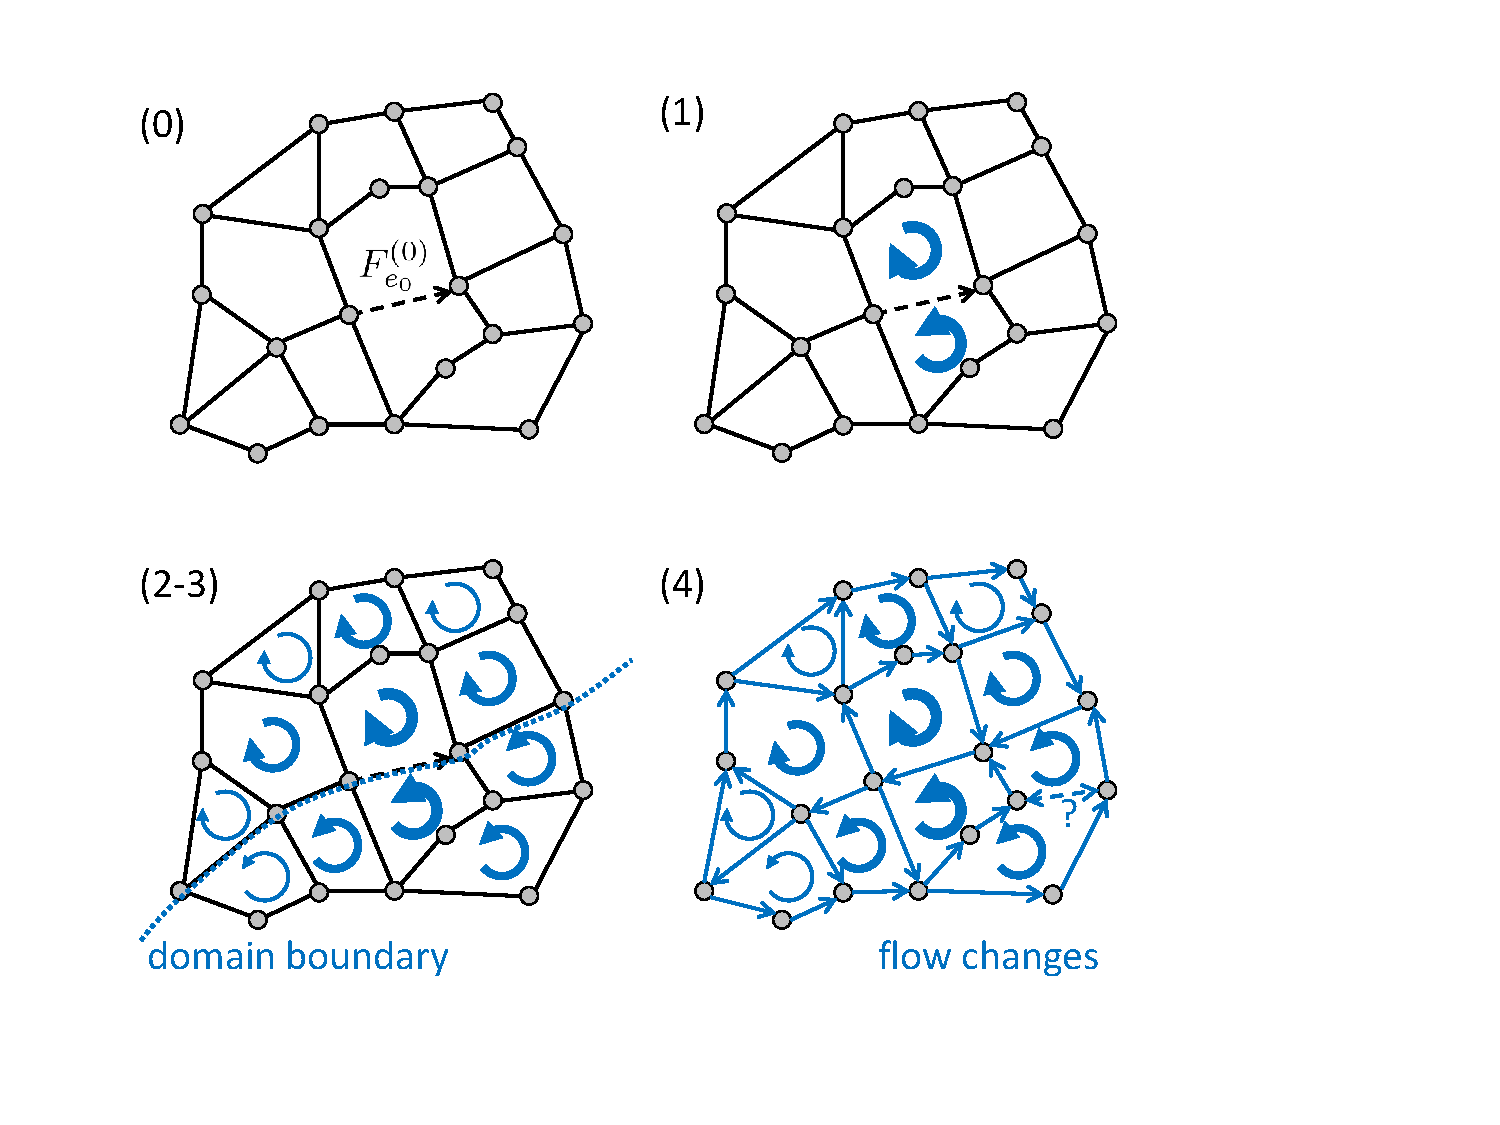
\includegraphics[trim=2cm 2cm 7cm 3cm, width=8cm]{pics/scheme1.pdf}
%\includegraphics[width=8cm]{pics/scheme30.pdf}
\caption{
\label{fig:scheme}
Schematic representation of the algorithm \ref{thm:alg1} to predict
flow changes after the damage ($\kappa < 0$) of a single edge (dashed).
}
\end{figure}

We note that $d$ denotes the distance of two cycles or faces, i.e. the length of the shortest 
path between the two faces in the dual graph. A proof is given in appendix \ref{sec:proof2}. 
Strict monotonicity can be proven when some additional technical assumptions are satisfied, 
which is expected to hold in most cases. In fact, one finds that the decay is rather fast for 
many networks of interest:

(1) For two-dimensional lattices with regular topology and edge weights the cycle flows decay with the inverse distance. A proof for square lattices in the continuum limit is given in appendix \ref{sec:proof-regular}.

(2) For two-dimensional lattices with regular topology but disordered edge weights, the eigenstates of $A$ generally decay exponentially with the euclidean distance. This statement is a manifestation of Anderson localization and was confirmed numerically for many random network ensembles \cite{Kram05,Huan09,Kett12,Laba14}.
\footnote{In lattices with subgrid symmetry states exist which decay exponetially with the square root of the distance.}.  
  
These results imply that the cycle flows $|f_c|$ decay rather rapidly with the distance such that the reponse of a supply network is confined to the `vicinity' of the damaged edge. However, it has to be noted that the distance is defined  for the dual graph, not the original graph, and that the rigoros results hold only for planar graphs. The situation is much more involved in non-planar graphs, as an edge can link regions which would be far apart otherwise.

We are thus in the position to predict the change of network flows after the perturbation of a single edge
on a purely topological basis according to the following algorithm whose steps are illustrated in figure \ref{fig:scheme}.

\begin{alg}
\label{thm:alg1}
(Prediction of flow changes)
\begin{enumerate}
\item
Assign a cycle flow to the cycles directly adjacent to the perturbed edge $e_0$, denoted by $c_1$ and $c_2$ in the following. If $\kappa < 0$, these cycle flows are anti-parallel to $F^{(0)}_{e_0}$, if $\kappa > 0$ the cycle flows are parallel to $F^{(0)}_{e_0}$.
\item
Assign a cycle flow with the same orientation to all cycles adjacent to $c_1$ and $c_2$. If a cycle is adjacent to both $c_1$ and $c_2$, the flow direction for this cycle cannot be decided. Assume that the strength of the cycle flow is weaker. 
\item
Repeat this for the next-to-nearest neighbors and so on.
\item
The direction of flow change of each edge is then given by the direction of the strongest cycle flow in the two adjacent cycles. The flow over a bridge and the flows in disconnected cycles remain unchanged.
\end{enumerate}
\end{alg}

%\begin{figure}[tb]
%\includegraphics[width=6.5cm]{pics/detailed_perturbation-7.png}
%\includegraphics[width=8cm]{pics/detailed_perturbation-11.png}
%%\includegraphics[width=6cm]{pics/detailed_perturbation-10.png}
%%\includegraphics[width=6cm]{pics/detailed_perturbation-9.png}
%\caption{
%\label{fig:leaf1}
%Cycle flows induced by the damage of a single vein in the vascular network of a leaf.
%The network consists of two connected domains with clockwise (blue) and
%counter-clockwise (red) cycle flows, as described by proposition \ref{thm:domains}
%The strength of the flows, indicated by the cycle radius, decays rapidly with the 
%distance to the damaged vein.
%Shown are results of a numerical simulation based on real-world leaf data
%as described in \textbf{[XXX]}. The lower plot show a blow-up of the leaf
%around the perturbed vein.
%}
%\end{figure}

\section{Linear flow in Planar graphs}
\label{sec:linflow-planar}

In many important applications the flow is directly proportional to the
potential drop along an edge of the network.
Then the equation for the cycle flows (\ref{eqn:cflow-lin}) becomes exact,
with $g \equiv 1$ and the matrix $A$ given by 
\begin{align}
   \label{eqn:lin-Lapldef}
   A_{d,c} &= \sum_{e=1}^L C_{d,e} C_{c,e} \\
           &=
	     \begin{cases}
	     \text{No. of edges shared by faces c and d} & \text{if } c\neq d\\
	     \text{No. of edges in face c} & \text{if } c=d.
	     \end{cases}
    \nonumber	     
\end{align}
Hence, the matrix $A$ can be seen as a part of the Laplacian of the dual  
of $G$, the original network, excluding the row and column corresponding to 
the unbounded face of $G$. A formal solution of Eq.~(\ref{eqn:cflow-lin}) 
shows that the induced cycle flow $f_c$ depends on the toplogy of the 
network only via the so-called `resistance distances' $R$ to the cycles
$c_1$ and $c_2$,
\begin{align}
    \label{eq:fc-resdist}
   f_c &\propto R_{c,c_1}-R_{c,c_2}
\end{align}
(for derivation see Appendix \ref{sec:resdist}).
Resistance distances have been first introduced for networks of electric resistors,
where they describe the effective resistance between two nodes \cite{Klei93},
and provide a metric on graphs.
\dirk{XXX @ Debsanka: That't nice, but what is it good for? XXX}

Now we discuss how the decay of cycle flow differs in different network 
topologies.  

To analyze how the topology affects the response of a flow network, in particular
its decay with the distance, we simulate the flow change for a collection of regular and 
random lattices. 
For a square lattice, we find that the cycle flows are approximately proportional to the 
inverse distance from the source of the perturbation. Near the boundary of the finite
network, decay becomes much more rapid (Figure \ref{fig-decay-sqlat}). 
Topological randomness is introduced by merging a nodes with a randomly chosen 
neighbours with a small probability $p$.  As we see in figure \ref{fig-decay-2p}, the 
introduction of randomness slows down the decay of cycle flows.  
However, as we see in figure \ref{fig-decay-2p-inv}, there still exists a 
region extending from the source of the perturbation till ~$40$\% of the 
diameter of the graph where the decay of cycle flow is linear.  


\dirk{XXX Can we please show all results in one figure? Left: Flow strength in color code
for a map of the lattice as in the paper by Kettemann et al. Right: Magnitude $|f_c|$ versus
distance without, with small and with strong randomness. And if you want to show an 
algebraic decay, please use a double-logarithmic plot. Make a statement if the numerical 
findings are consistent with the analytic results in appendix \ref{sec:proof-regular}.
And please see my notes  about the the appropriate length scale below...}

\begin{figure}
    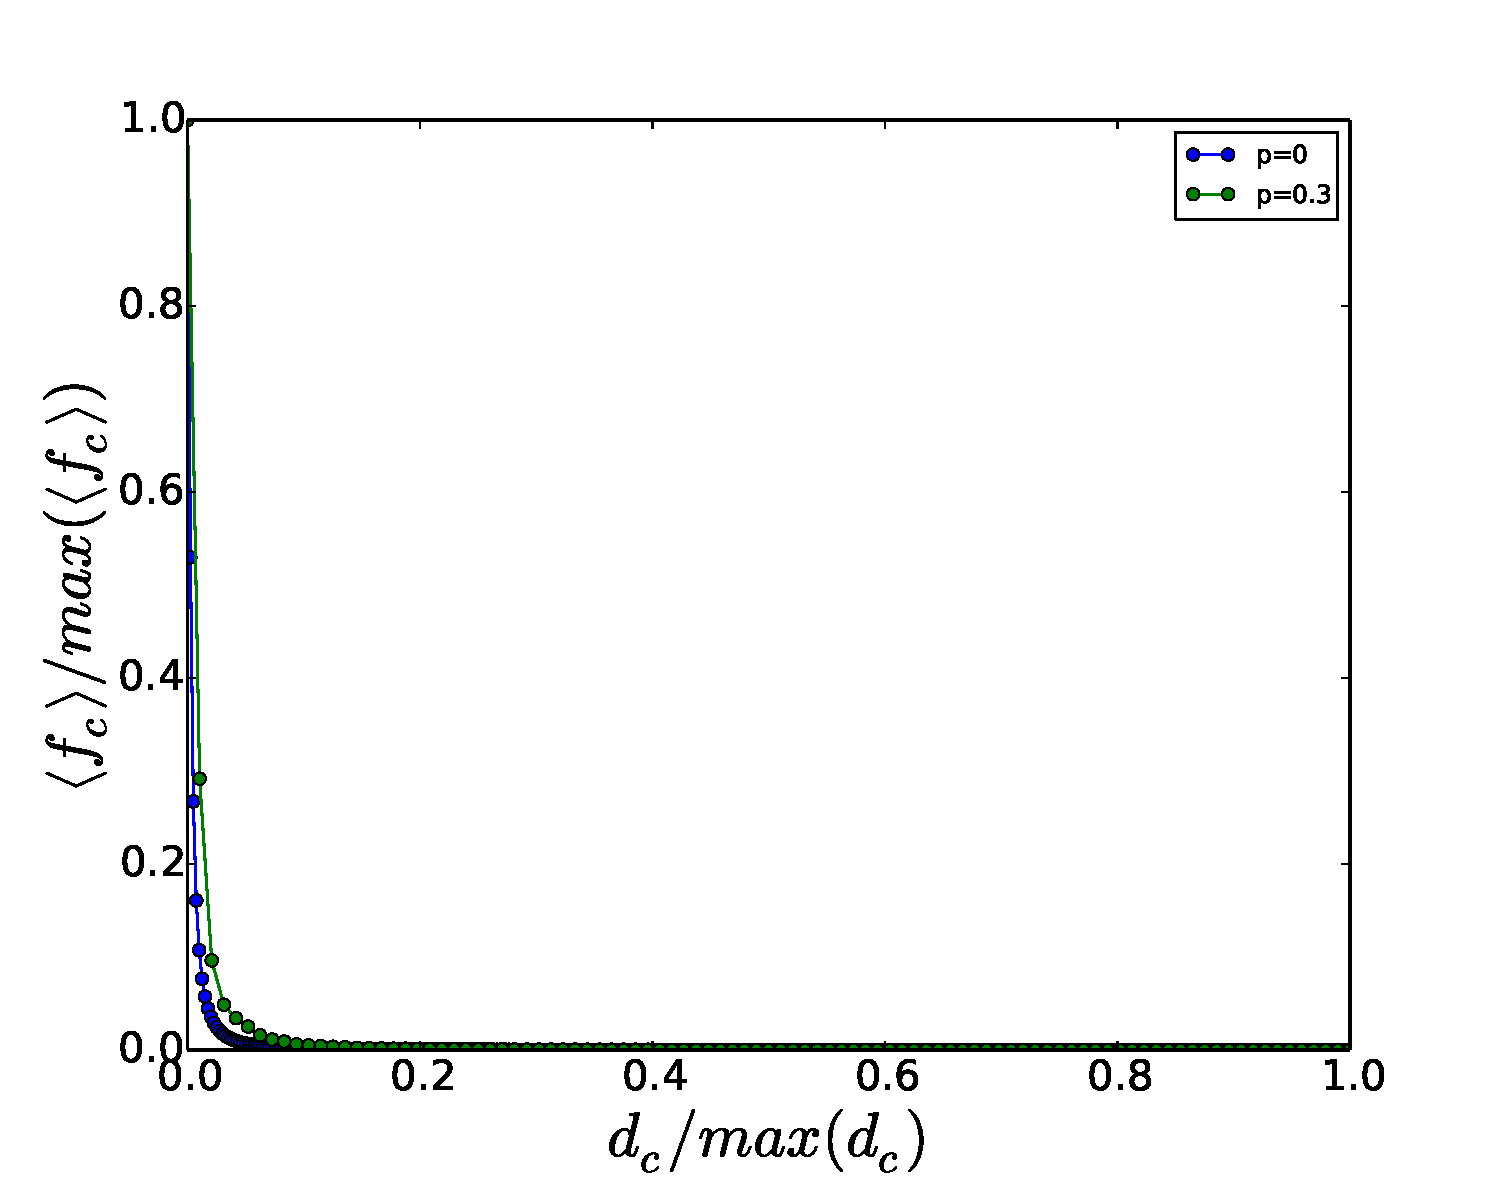
\includegraphics[width=.9\columnwidth]{pics/decay_sqgrid}
    \caption{Decay of induced cycle flows in a square lattice of size 200x200 after the 
        failure of the edge edge between nodes (0,0) and (0,1).}
    \label{fig-decay-sqlat}
\end{figure}


\begin{figure}
    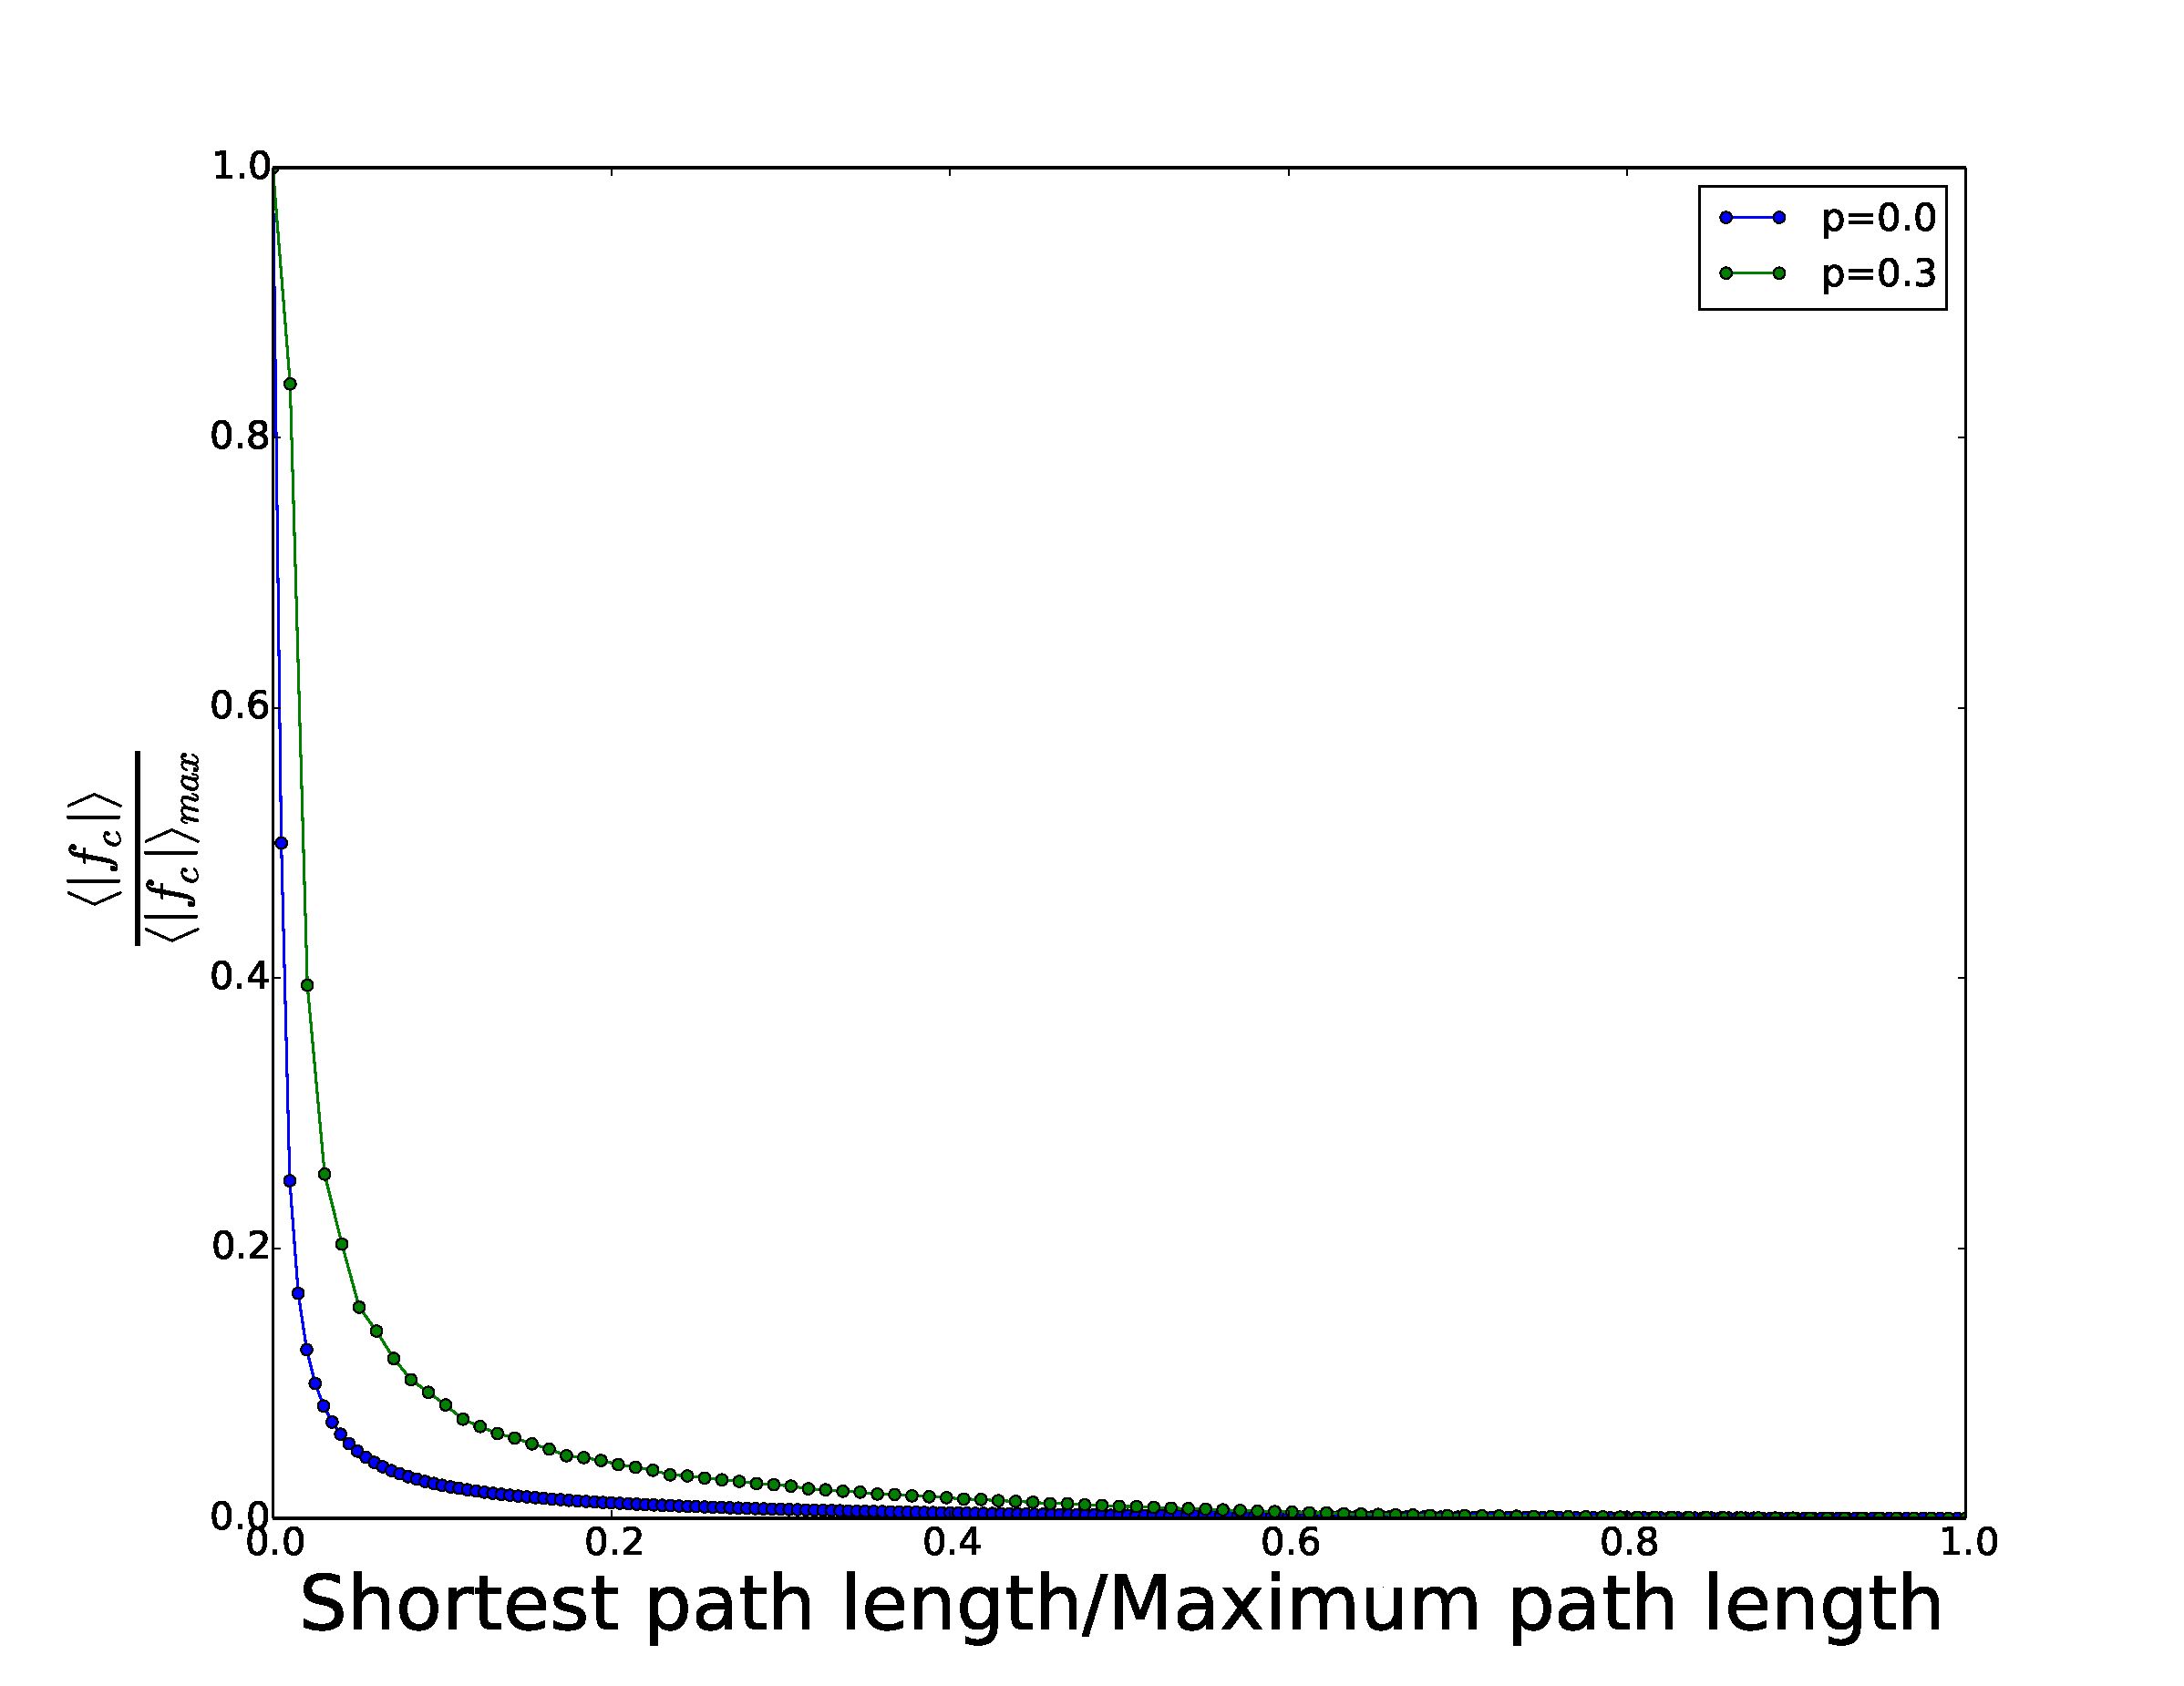
\includegraphics[width=.9\columnwidth]{pics/decay_2p}	
    \caption{Decay of cycle for in a square lattice with randomness factor $p$}
    \label{fig-decay-2p}
\end{figure}

\begin{figure}
    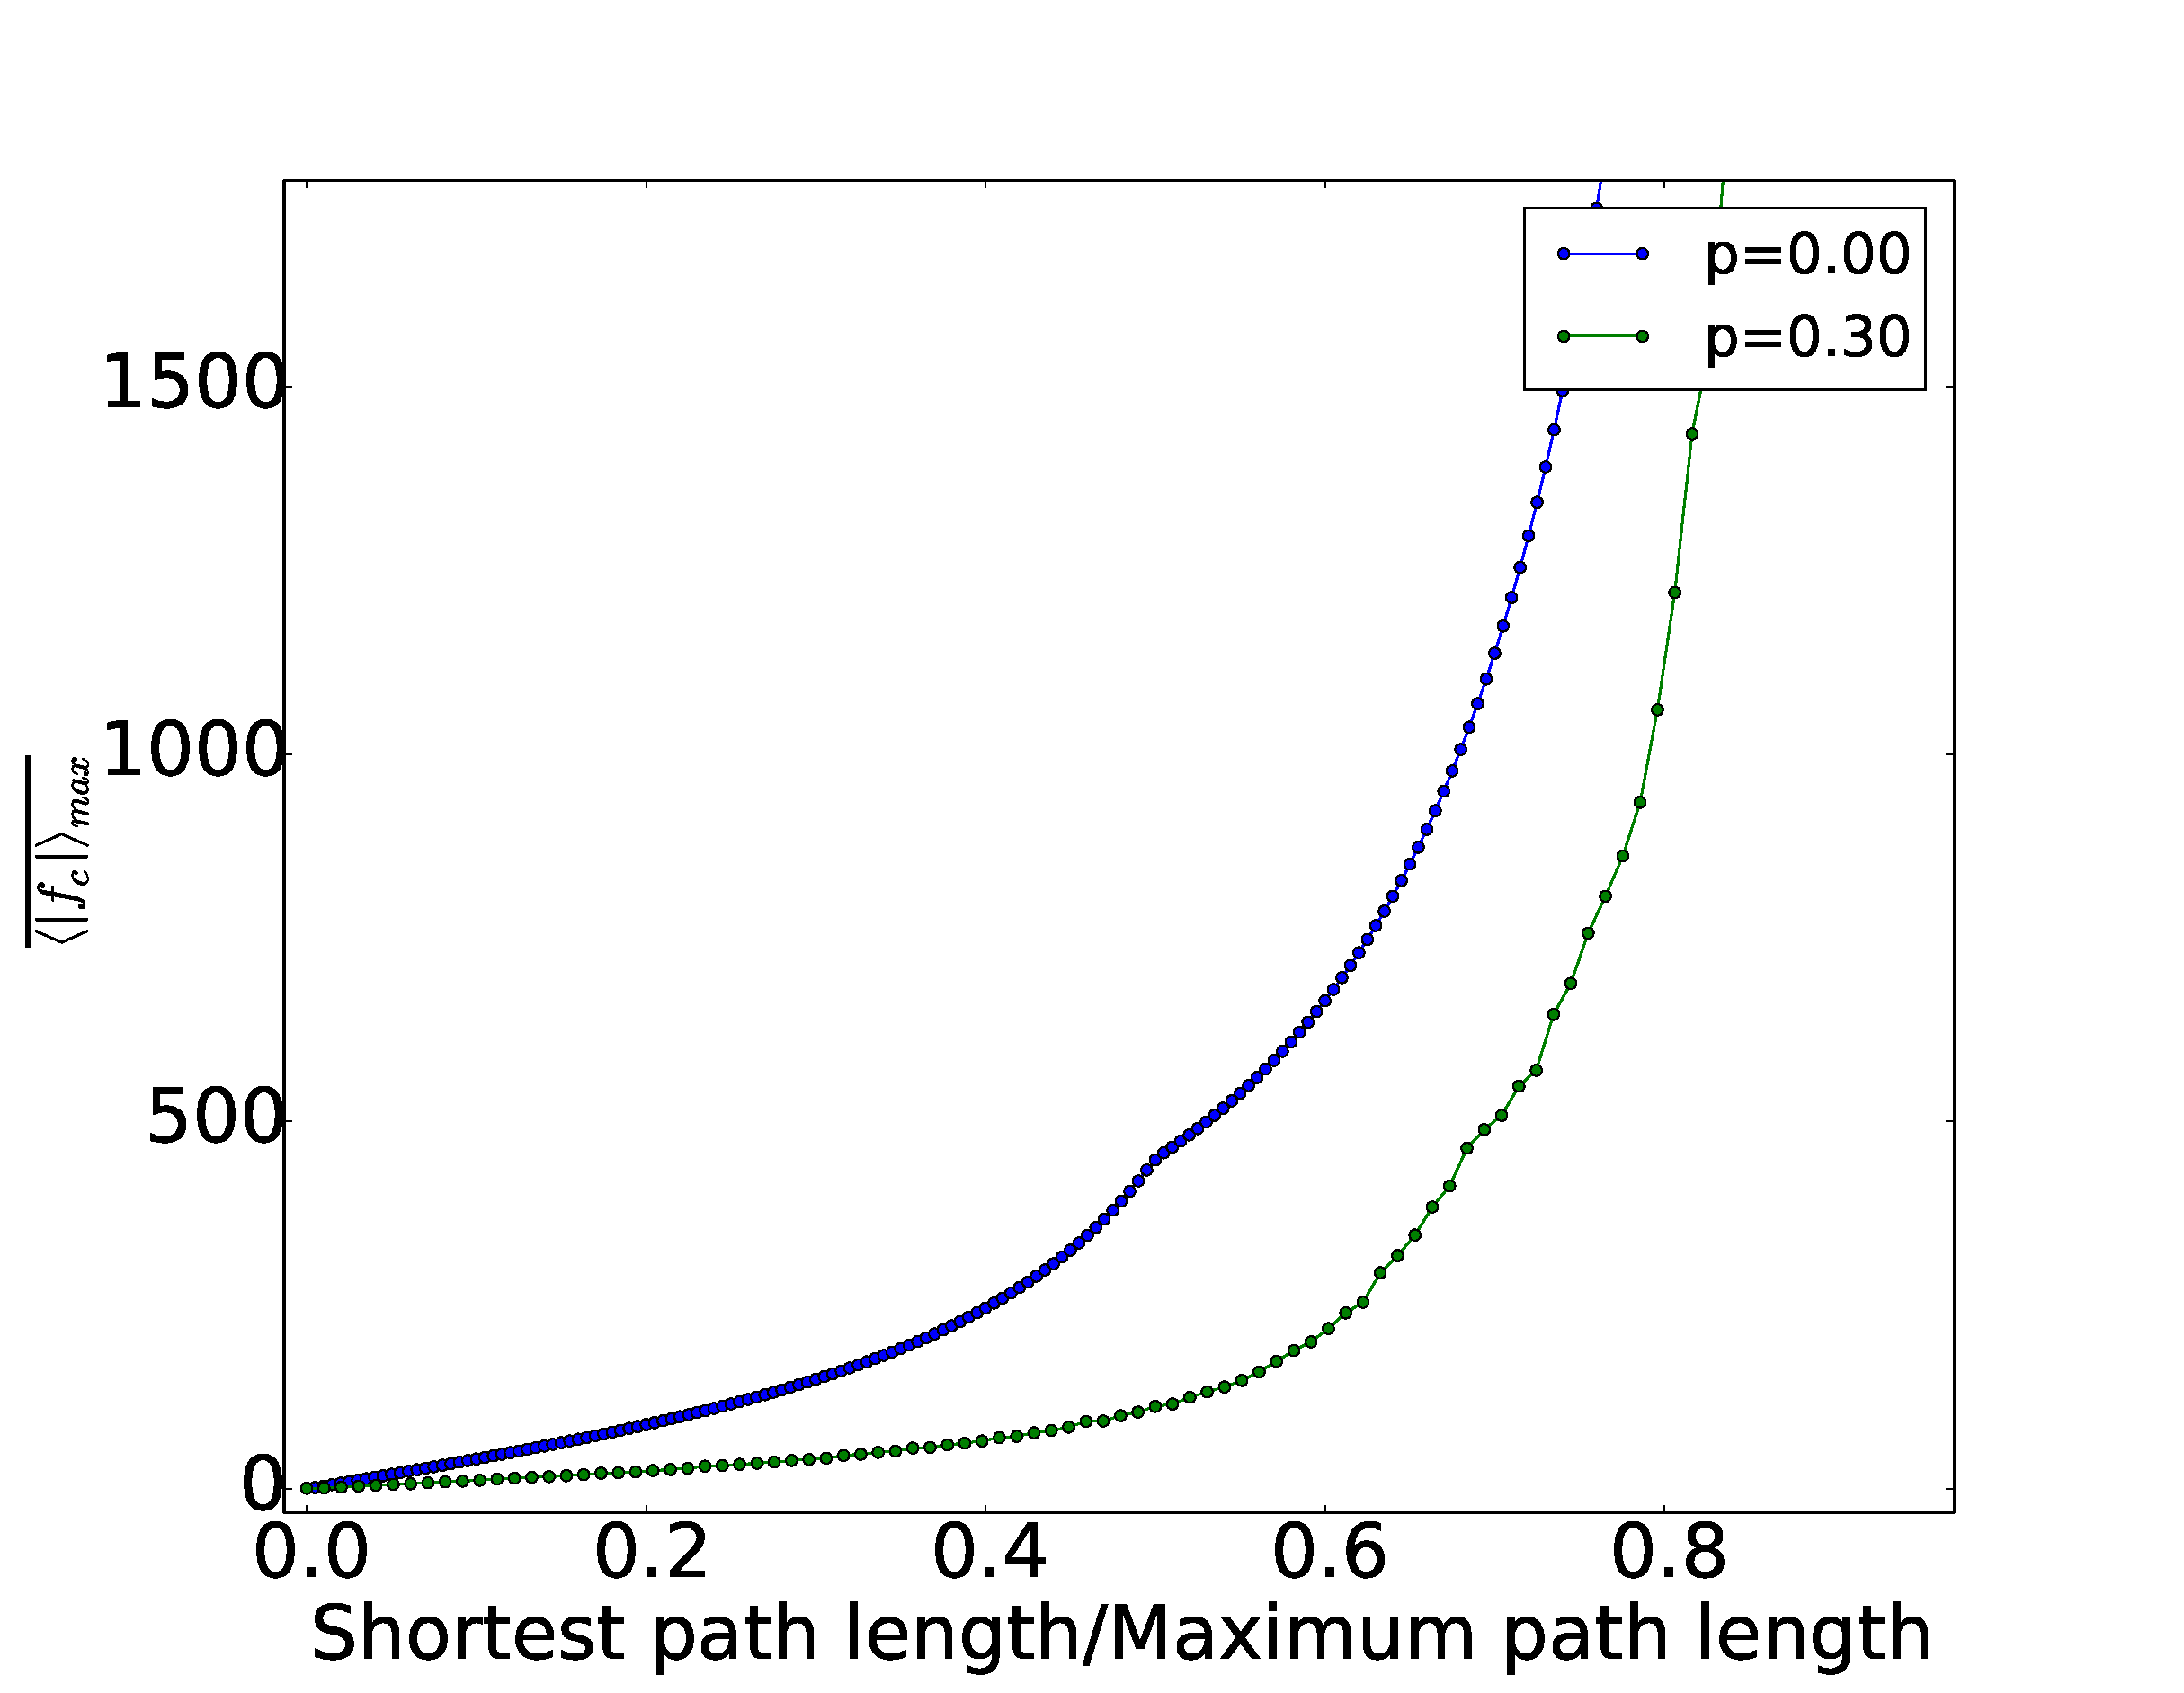
\includegraphics[width=.9\columnwidth]{pics/decay_2p_inv}	
    \caption{Inverse of $f_c$ for in a square lattice with randomness factor $p$}
    \label{fig-decay-2p-inv}
\end{figure}


\dirk{
Dear Henrik and Debsankha, I have two comments on your results. 
(1) In a previous version I recommended to show that the induced cycle flows are 
proportional to the initial flow of the failing edge. You have argued that this is trivial 
since the entire system is linear anyway. 
But this assumption is only partially true. If you vary the strength of the perturbation
$\kappa$ at \emph{a fixed edge} then the response is trivially propotional to $\kappa$.
And also if you vary $F_e^{(0)}$ for \emph{a fixed edge} the response will be 
trivially proportional to $F_e^{(0)}$. That's what the equations (\ref{eqn:cflow-lin}) 
and (\ref{eqn:def-A}) tell us, assuming that the system is linear such that the function 
$f$ is the identity such that the function $g$ uis constant.
However, I claim something which is much stronger. My numerical test with the power 
grids show that the reponse is proportional to $F_e^{(0)}$ \emph{regardless of which
edge fails}. The only thing that matters is the cycle distance between failing edge and
the observed edge, where you measure the perturbation. For a cycle distance $d_c=0$
the proportionality factor is one and the correlation is almost perfect. That is what I show 
in figure \ref{fig:case30q}.
It't not so easily to clearly explain the difference and to show its importance. But I do thing
that it is very important since it shows the \emph{universality} of our concept. All the 
topology is not so interesting after all. In the moment I think that we should illustrate this
result in the section on random networks, but I am not sure.
}

\dirk{
(2) The second important question is what I tried to make clear on the telephone: What
is the important length scale in a flow network. I argue that it is not the usual edge 
distance of two edges but the \emph{cycle distance} of two edges. I give a rigorous 
definition below. Basically $d_c(e_0,e_1) = 0$ means that the two edges $e_0$ and $e_1$ 
are on the same cycle. I claim that all edges  $e_1$ with $d_c(e_0,e_1) = 0$ are equally 
affected when the edge $e_0$ fails, regardless of their edge distance! For the power grid 
example this claim definitely holds as shown by the perfect correlation coefficient in
(see figure \ref{fig:case30q} c). Open questions are: Does this hold generally also for 
random networks? Does it hold also for larger edge distances? To answer these two question 
we should simulate random planar networks with cycles of very different size and analyze 
which distance metric (edge vs. cycle) better predicts the decay of the response. I can think 
of different options to do so, and maybe you find an even better option:
(a) Do plots as in figure \ref{fig:case30q}, once with the cycle distance and once with
the edge distance. I assume that the correlation factor $R$ is much  higher for the cycle 
distance.  
(b) Directly plot the normalized reponse $\Delta F_{e'}/F^{(0)}_e$ as a function of the
distance between $e$ and $e'$ and analyze the correlation by means of the correlation 
ratio or the mutual information, or I don't know. You have many experts on measuring 
correlations at MPI DS.
}


\textbf{Definition of cycle distance:}
The strength of the cycle flows is expected to decay rapidly with the distance, which has to be 
understood as the graph-theoretic distance in the \emph{dual} graph (called $d_d$ in the following).
Therefore also the change of the edge flows after a perturbation,
\be
   \Delta F_e = F'_e  - F_e^{(0)} = \sum_{c=1}^{L-N+1} f_c C_{c,e},
\ee
is expected to decay rapidly, where the relevant distance is still determined by the adjacent 
cycles. We thus define the cycle distance of two edges $e_0$ and $e_1$ as the minimum distance 
of the adjancent cycles in the dual graph, 
\be
  d_c(e_0,e_1) = 
  \begin{cases}
      0 & \text{if } |C_{c,e_0}| = |C_{c,e_1}| \,  \forall c \\
      \min \limits_{\substack{c_0,c_1 \text{ s.t.} \\  |C_{c_0,e_0}| = 1 \\  |C_{c_1,e_1}| = 1}} 
          d_d(c_0,c_1) +1
      & \text{otherwise.} \\
  \end{cases}
  \label{def:cycledist}
\ee
We note that this distance can be strongly different from the common edge distance
(called $d_e$ in the following), which is defined as the length of the shortest path from
$e_0$ to $e_1$ in the repective line graph.

\dirk{One remark. Maybe we should slightly change the definition by adding 1 to the formula
\ref{def:cycledist} and defining $d_c(e,e) = 0$. Then we have a real distance in the mathematical 
sense. At least I hope so. We would still have to check the triangle inequality.}


\section{Vascular networks}


Vascular plants possess an intricate, highly reticulate network 
supplying the leaf blade with water for gas exchange through
evaporation as well as photosynthesis.
The transport of water in these vascular networks can be described by a 
potential flow as shown in \cite{Kati10}.
As leaf networks are naturally planar, our theorem can be 
used to predict the direction of flow changes after a damage to the leaf.

We demonstrate this by simulating the cycle flow arising from perturbing
the main vein of one leaf of Norway maple (\emph{Acer platanoides}).
The leaf was chemically cleared and stained to make the complete network
visible, then scanned at high resolution (3200 dpi) and the vascular
network extracted using a vectorization approach. The result is a
complete representation of the network topology and geometry.
\dirk{XXX Reference? XXX}

\begin{figure}
    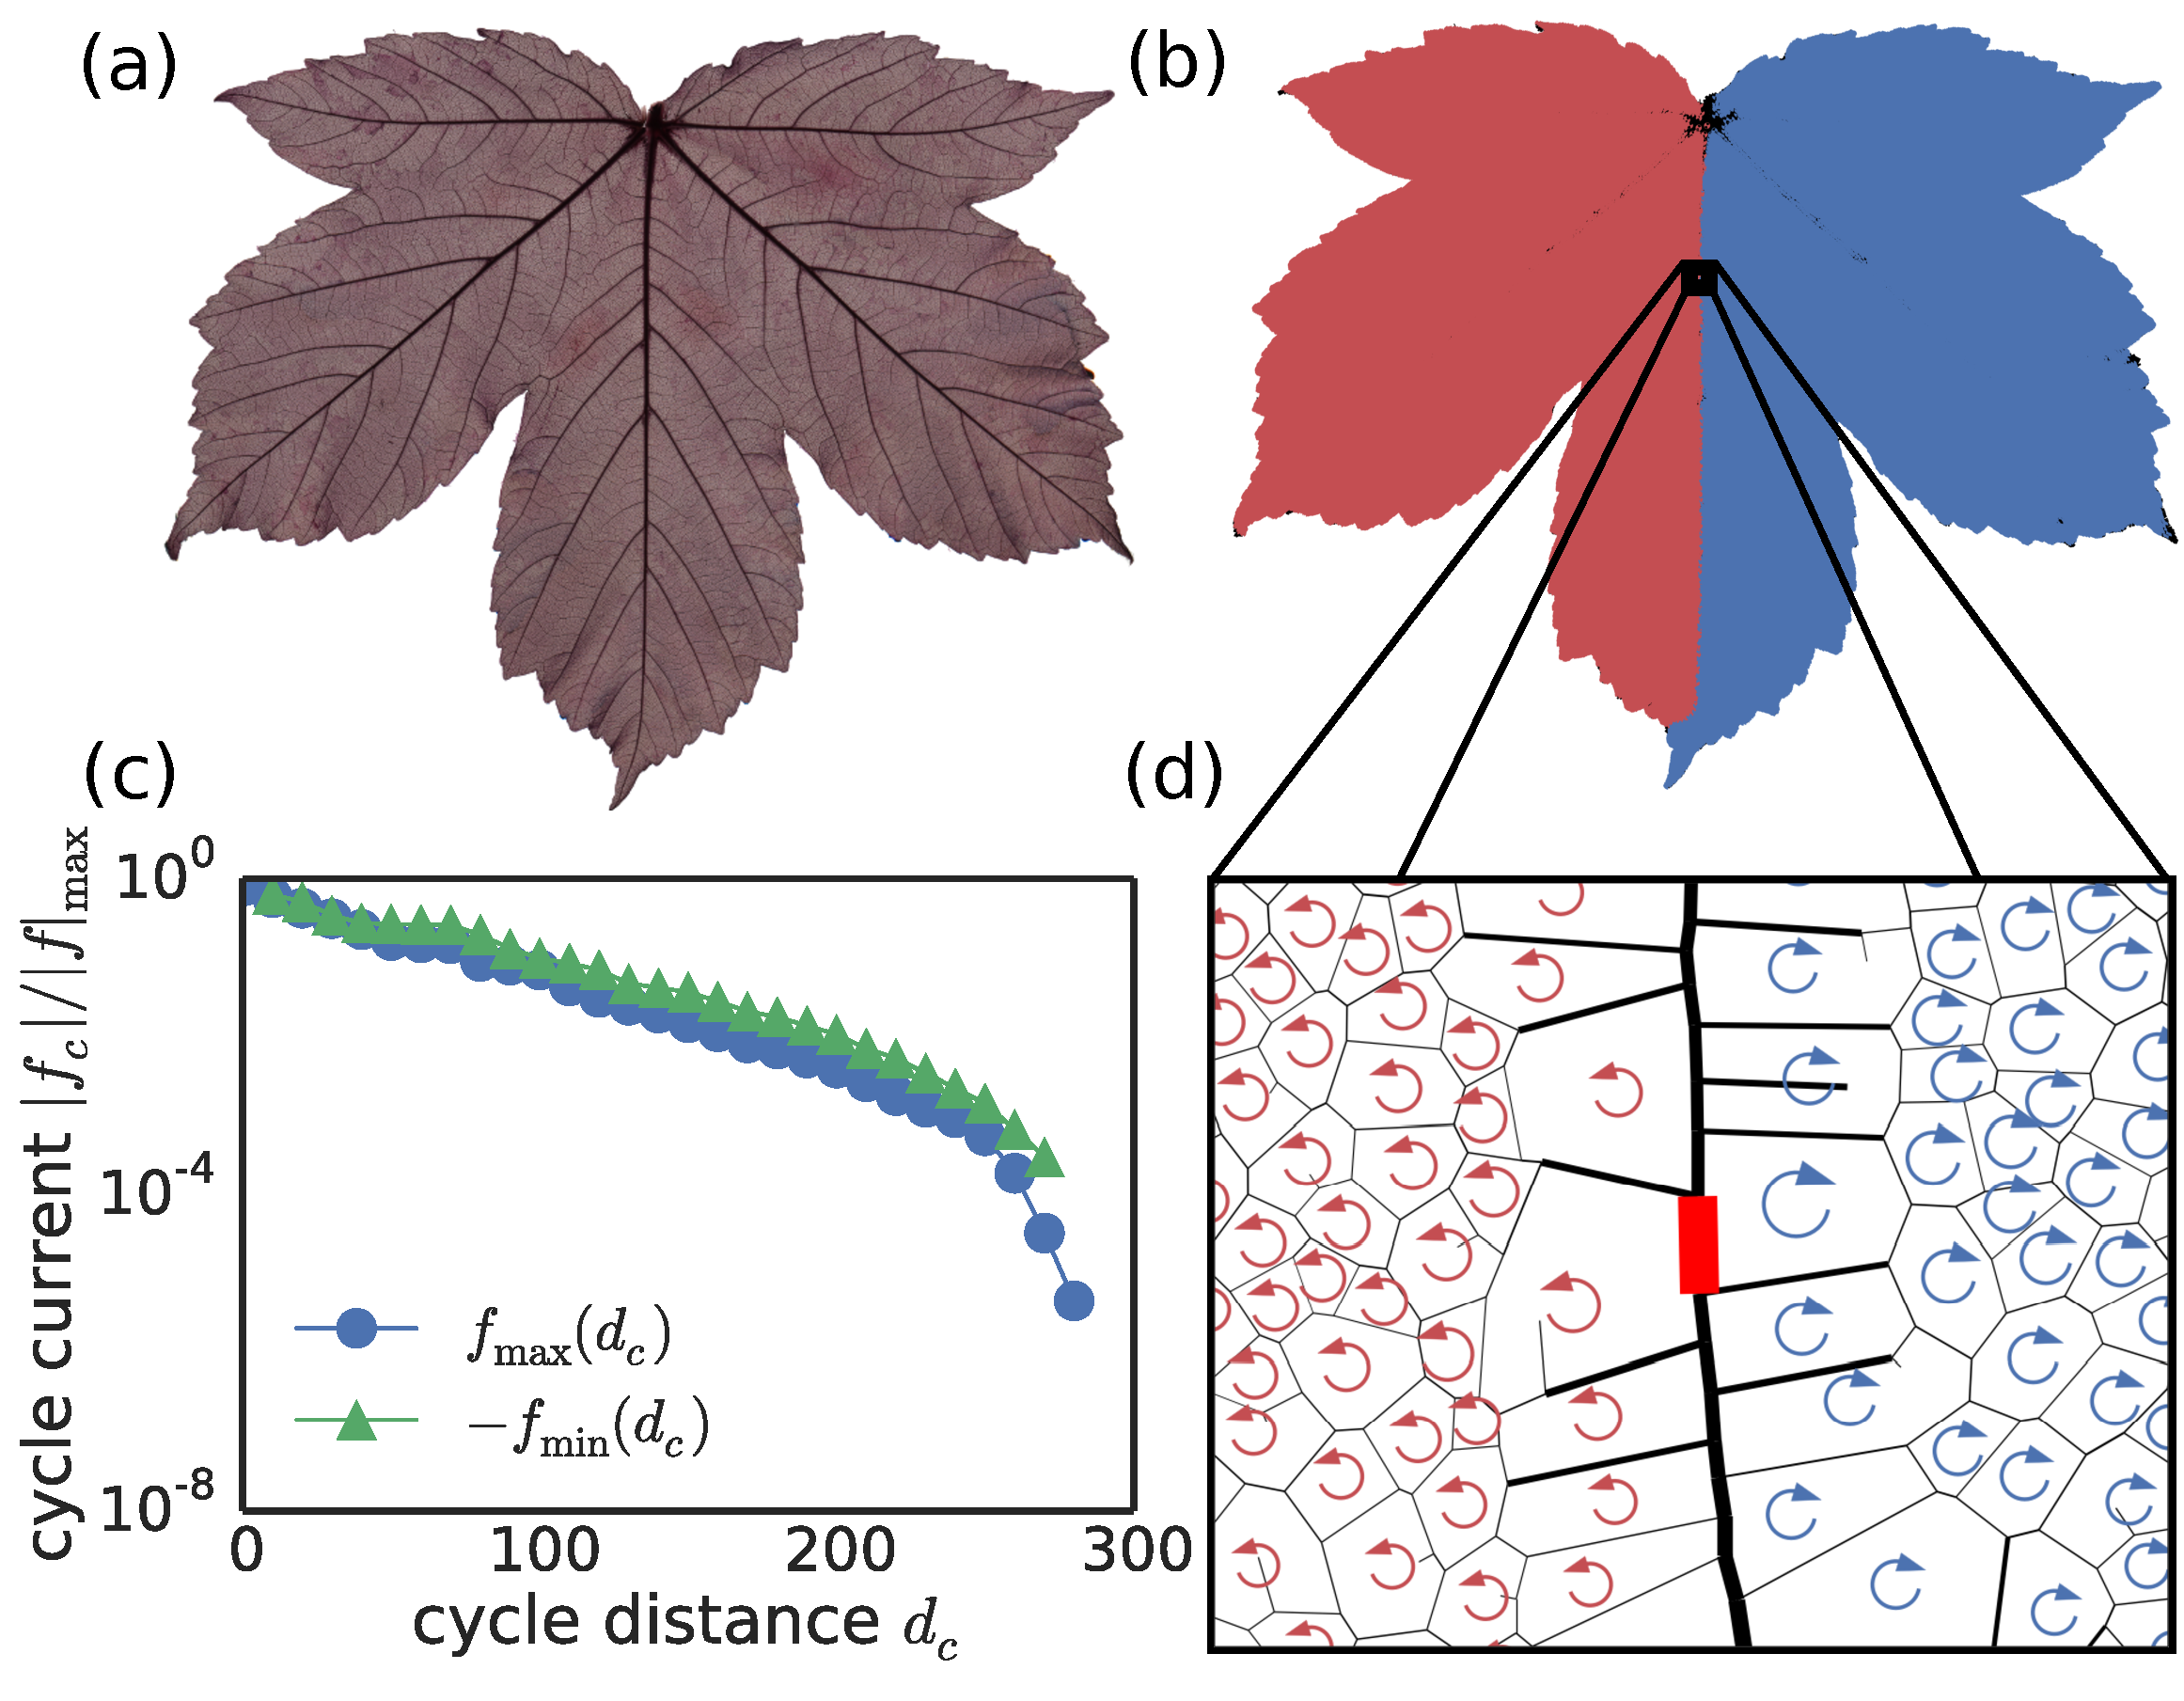
\includegraphics[width=.9\columnwidth]{pics/figure_simulations.pdf}
    \caption{(a) A leaf blade of Norway maple (\emph{Acer platanoides}),
    high resolution scan (3200 dpi). The complete venation network
    up to all orders was extracted from this image.
    (b) The flow network as extracted from the high resolution scan.
    One edge on the main vein has been perturbed (approximate position
    shown by black rectangle),
    oppositely oriented cycle flows are marked in red and blue.
    The domain boundary clearly follows the main vein almost perfectly.
    (c) A semi-logarithmic plot of the absolute value of maximum (blue
    circles) and minimum (green triangles) cycle flow strength as a 
    function of shortest path distance
    on the dual graph $d_c$ from the perturbation. Formally,
    $f_\mathrm{max}(d_c) = \operatorname{max}_{d(c', c_{e_0}) = d_c}
    f_{c'}$, where $c_{e_0}$ is one of the cycles adjacent to the 
    perturbed edge $e_0$ and $d(c,c')$ is the shortest path distance
    between cycles $c$ and $c'$ in the dual network. 
    The definition of $f_\mathrm{min}$ is similar.
    \dirk{XXX Can we please use the same definition as in the text, in particular
    proposition \ref{thm:decay} and just refer to it? XXX}
    Solid lines act as a guide for the eye.
    Decay is approximately exponential, showing strong localization 
    of the perturbation,
    compatible with results from Anderson localization.
    (d) Zoom to the region close to the perturbation. The perturbed edge
    is marked in bright red, oppositely oriented cycle currents are
    represented by oriented arrows. Arrow size is proportional to
    cycle flow magnitude, edge diameters are proportional to measured
    vein diameters but have been downscaled to improve clarity of the
    image.
    \dirk{XXX Can we have one sentence in the beginning summarizing the 
    main message of the figure and can we make the entire caption a bit shorter
    and more to the point? XXX}
    \label{fig:vascular-network}}
\end{figure}

Flow through an edge is described by $F_e = k\frac{R_e^4}{L_e} (p_{e_0}
-p_{e_1}$, where $R_e$ is edge radius, $L_e$ is edge length, $p_{e_i}$
is hydrostatic pressure at node $e_i$, and $k$ is a constant of 
proportionality. This is basically Poiseuille's law.\footnote{Recent
work has shown that in reality, there a scaling relationship between
effective hydraulic diameter $d_\mathrm{eff}$ and external vein diameter
$R$, $d_\mathrm{eff} \sim R^{1-\gamma/4}$ with $\gamma \approx 0.6$.
The radius parameter in Poiseuille's law should therefore really by
corrected in this way. However, this relationship is not relevant for
the point of this paper.}
The continuity equation is $\sum_e E_{i,e} F_e = P(1 + (N-2)\delta_{i,0})$,
modeling uniform evaporation of water over the whole leaf blade 
except at the petiole ($i=0$), which acts as an inlet.
\dirk{XXX Can we use $\phi$ for the pressure as before and $r$ for
the radius? We already have capital $R$ for the resistance distance. XXX} 

Since the flow equation is linear in the pressure difference, the
flow change due to the perturbation is indeed exactly 
(up to a constant factor) described by equation (\ref{eqn:cflow-lin}).
The simulation results are shown in figure \ref{fig:vascular-network}.
It is interesting to note that (a) the domain boundary between cycle
flows of opposite orientation follows the leaf symmetry axis (the main
vein) almost exactly. When perturbing other veins, the domain boundary
similarly appears to follow the locally thickest veins.
\dirk{XXX Cool. Can we have a few more pictures of different leaves 
demonstrating this result for the appendix? XXX}
Additionally, (b) cycle flow strength on either sides of thick veins
appears to jump when there is no domain boundary, effectively confining
the perturbation to a localized region.
A different localization behavior (c) can be observed by plotting
maximum and minimum cycle flow as a function of shortest path distance
on the dual graph. 
\dirk{XXX That's what I call cycle distance. We should have a consistent
notation. And we shuld put the definition into the main text instead 
of the figure caption ;-) XXX}
Approximately exponential decay is clearly discernible
over large distances. The leaf network is thus disordered enough
to show Anderson localization of the perturbation.
We speculate that this may be functionally relevant for the plant,
as damage in one part of the leaf has only local effects, leaving
most of the rest functioning undisturbedly.
\dirk{XXX Cool Cool Cool. XXX}




\section{Predicting blackouts in power grids}
\label{sec:powergrid}

Power grids form the backbone of our technical infrastructure. Their stable operation is essential for our economy and everyday life \cite{Stro01,Pour06}. Generally, power grids must be operated such that they are resilient against the damage of a single transmission line (the so-called $n-1$ criterion \cite{UCTE04}). Still, local failures repeatedly induce global outages in periods of extreme loads \cite{Pour06}, which are expected to become much more likely in the future \cite{Pesc14}. Any fundamental result that predicts the effects of local failures is thus of great scientific as well as economic value.

\begin{figure}
    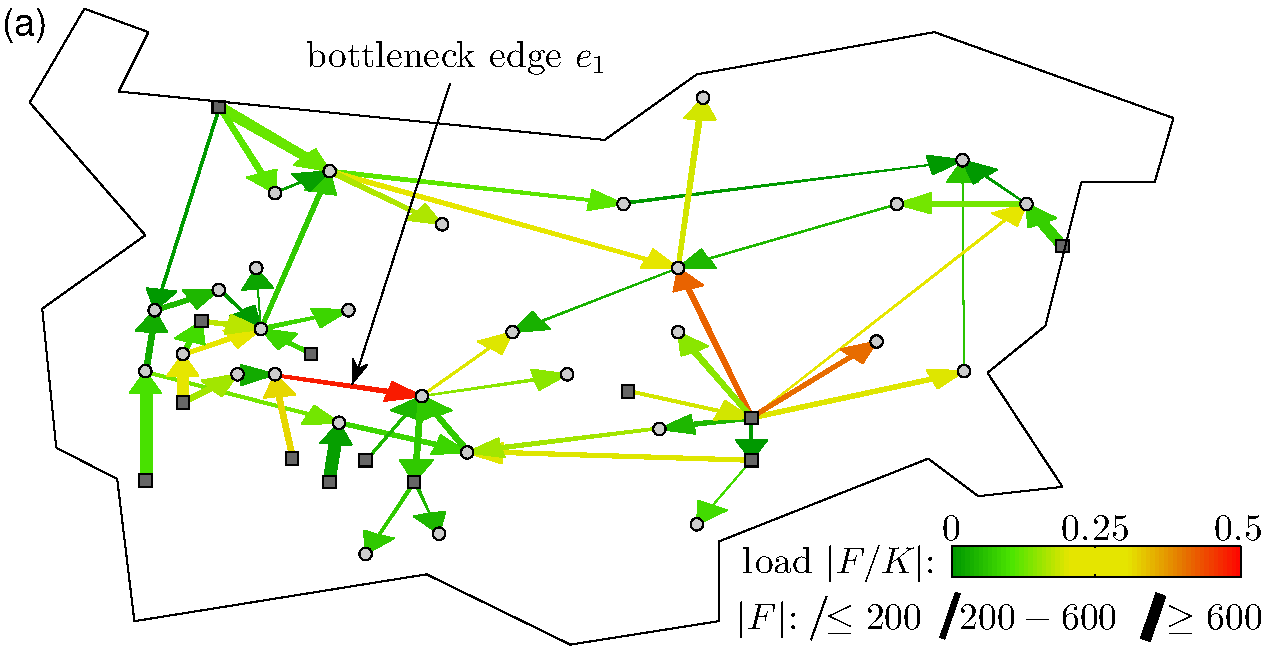
\includegraphics[width=\columnwidth]{pics/bulgaria15_iniload.pdf}
    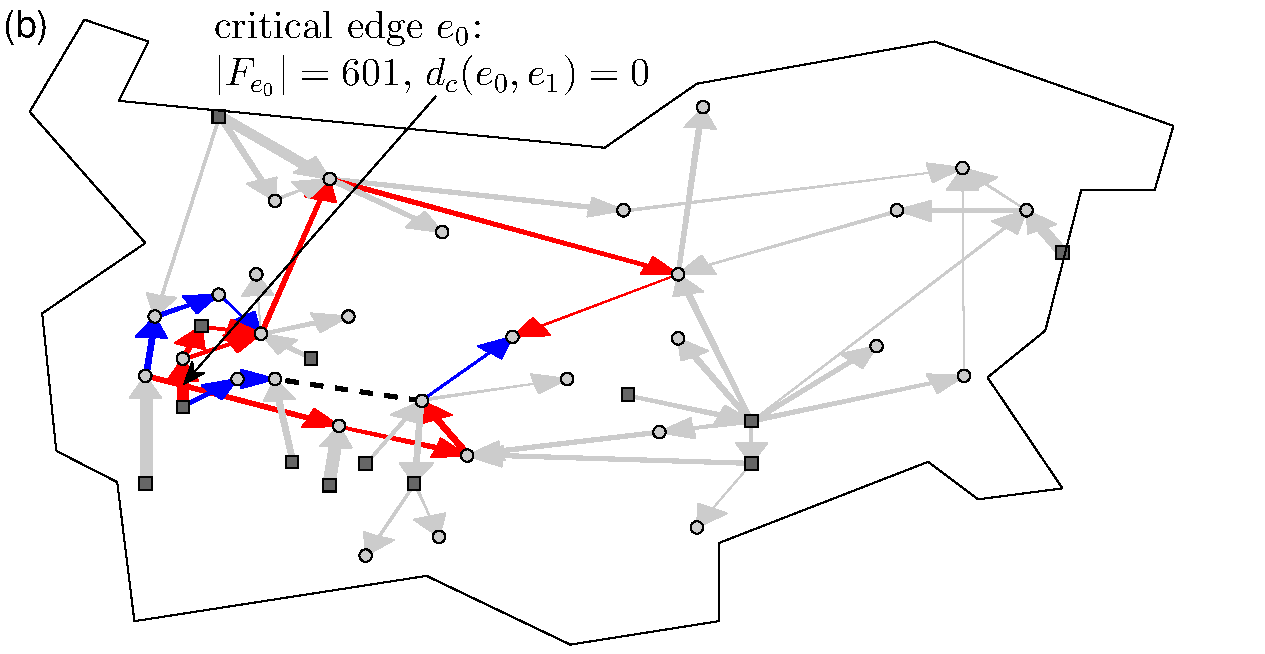
\includegraphics[width=\columnwidth]{pics/bulgaria15_change.pdf}
    \caption{\label{fig:bulgaria1}
    Indentification of critical transmission lines.
    (a) Model of the Bulgarian power transmission grid under extreme load (see text for details).
    Shown is direction and magnitude of the absolute power flow $|F|$ in MW as well as the
    relative load $|F/K|$ in a color code. One bottleneck edge $e_1$ in central Bulgaria 
    is vulnerable to secondary overloads.
    (b) Algorithm \ref{thm:alg1} readily predicts which outage will lead
    to an increase (red) or decrease (blue) of the flow on the bottleneck edge $e_1$. 
    Only edges with a small cycle distance $d_c \le 1$ are considered, as remote edges
    are expected to have no significant influence. In this way, one critical edge $e_0$     
    is identified which has a small distance $d_c(e_0,e_1) = 0$ and a high initial
    flow $|F_{e_0}| = 601$ MW. 
    }
\end{figure}

If ohmic losses can be neglected and the voltage magnitude $U$ is constant throughout the grid,
then the real power flow between two nodes $j$ and $\ell$ reads \cite{Wood13,12powergrid}
\be
      F_{j,\ell} =  U^2 B_{j\ell} \sin(\phi_{j} - \phi_\ell ),   
\ee
where $\phi_j$ is the power angle, i.e. the the phase angle of the complex voltage at
node $j$, and $B_{j \ell}$ is the admittance of the respective transmission line.
The continuity equation for the real power is given by (\ref{eqn:continuity1})
such that the our results can be used to analyze the consequences of transmission
line failures. The case of non-vanishing losses is further analyzed in appendix
\ref{sec:acohm}.
 
The topological response theory allows a direct assesment of transmission lines which are
critical for network operation in the sense that their failure might induce a cascade leading
to a network-wide outage. As an example, we analyze the operation of the Bulgarian power grid 
in a hypothetical situation of extreme load shown in figure \ref{fig:bulgaria1} (a). The network 
model is based on the dataset \cite{Hutc13}, neglecting power im- and exports and increasing 
the generation and load at all nodes by a constant factor 50 \% in comparison to the normal operation.
The grid is no longer $n-1$-secure in this situation.  Can we predict which transmission line
failures can induce secondary outages and thus a potentially catastrophic cascade of failures?

To find the Achilles' heal of the grid, we face the \emph{inverse} problem as before. 
The starting point is the observation of one heavily loaded transmission line 
$e_1$ in central Bulgaria, which is vulnerable to secondary overloads
(see figure \ref{fig:bulgaria1} (a))
Then we have to calculate which perturbations in the grid would create the strongest response 
at the transmission line $e_1$.  
First, applying algorithm \ref{thm:alg1} to all possible trigger edges $e$ in the network 
reveals whether the load of $e_1$ increases or decreases when $e$ fails. It increases
when the flow change $\Delta F_{e_1}$ is parallel to the inital flow $F_{e_1}^{(0)}$,
and decreases otherwise.
Second, we have shown that the strength of the flow change are essentially determined by the 
initial flow of the failing edge and the cycle distance. In the current example we thus identify 
a single transmission lines with a cycle distance $d_c(e_0,e_1)=0$ and a hight initial flow
$|F_{e_0}^{(0)}| = 601$ whose failure is predicted to increase the load at $e_1$ 
(see figure \ref{fig:bulgaria1} (b)). Indeed, numerical simulations confirm that exactly this 
edges $e_0$ is indipensible for network operation. If is fails, no solution of the continuity 
equation can be found, which signals an impeding blackout of the grid. 

Notably, we also find several edges, whose removal would \emph{reduce} the load of the vulnerable
edge $e_1$. Hence, the removal of a transmission line can be beneficial as it decreases the 
maximum load in the grid. This surpring behaviour has been first discussed by Braess for
traffic networks in a game theroretic framework \cite{Brae68} and has recently been 
generalized to other types of supply network \cite{Mott04,12braess,13nonlocal}  
The topological response theory provides an intutive explanation of this behaviour
and shows that it is rooted in the cyclic topology of the network. In fact, it should
occur for all types of network that respect the continuity equation.
  

\section{Discussion}

\textbf{XXX TODO XXX}

\acknowledgments
 
We gratefully acknowledge support from the Helmholtz
Association (grant no.~VH-NG-1025) and the Federal Ministry of 
Education and Research (BMBF grant no.~03SF0472B and 03SF0472E).

\appendix

\section{Reponse theory for AC Power Grids}
\label{sec:acohm}

The state of an AC electric power grid is generally described by the so-called load flow equations
for the real and the reactive power. They include ohmic losses such that the continuity equation
(\ref{eqn:continuity1}) does not apply directly. However, the losses are generally small such that
topological response theory can still provide a very good prediction of the state of the grid after 
a transmission line failure. In this appendix we briefly introduce the load flow equations and 
analyze the performance of this prediction for a common model power grid.

Consider grid with $N_g$ generator nodes and $N_l$ load nodes. The continuity equation for the real power reads \cite{Wood13}
\be
      P_k = \sum_{m=1}^{N_g+N_l} U_k U_m
            \left( G_{k m}\cos \phi_{km}+B_{k m}\sin\phi_{km} \right),   
   \label{eqn:activepower}\\
\ee
where $P_k$ is the power generation or demand at node $k$, $U_k e^{i \phi_k}$ is the 
complex voltage and $\phi_{km} = \phi_k - \phi_m$ abbreviates the phase difference. 
The coupling of the nodes is described by the nodal admittance matrix 
$Y_{k m} = G_{km} + iB_{km}$. If all votages are constant, $U_k = U$ and ohmic 
losses can be neglected ($G_{km} = 0$), then we recover the continuity equation 
in the form discussed in section \ref{sec:continuity},
\be
      P_k = \sum_{m=1}^{N_g+N_l} U^2  B_{k m}\sin( \phi_{k} - \phi_m). 
\ee
These approximations are mostly satisfied in modern power grids. Even more, a linearization as in equation (\ref{eqn:cflow-lin}) is appropriate when the grid is not too heavily loaded, which yields the so-called DC approximation \cite{Wood13,Hert06}. Most power grids are approximately planar, crossings of transmission lines are possible but rare. We thus expect that the algorithm \ref{thm:alg1} can still predict the effects of the damage of single transmission lines in real power grids with great accuracy.

\begin{figure}[tb]
%\includegraphics[trim=0cm 4cm 0cm 0cm, width=8cm]{pics/case30_tot.pdf}
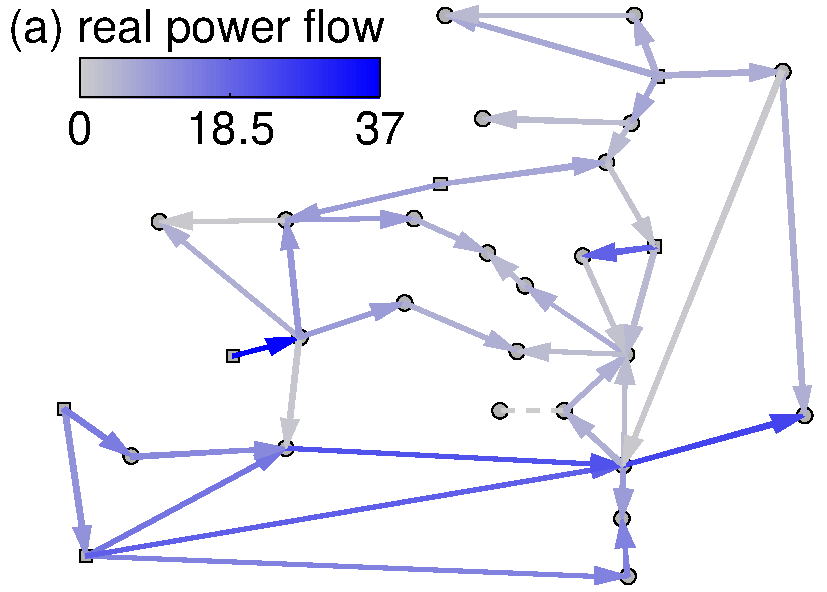
\includegraphics[width=4cm]{pics/case30c_flow2.pdf}
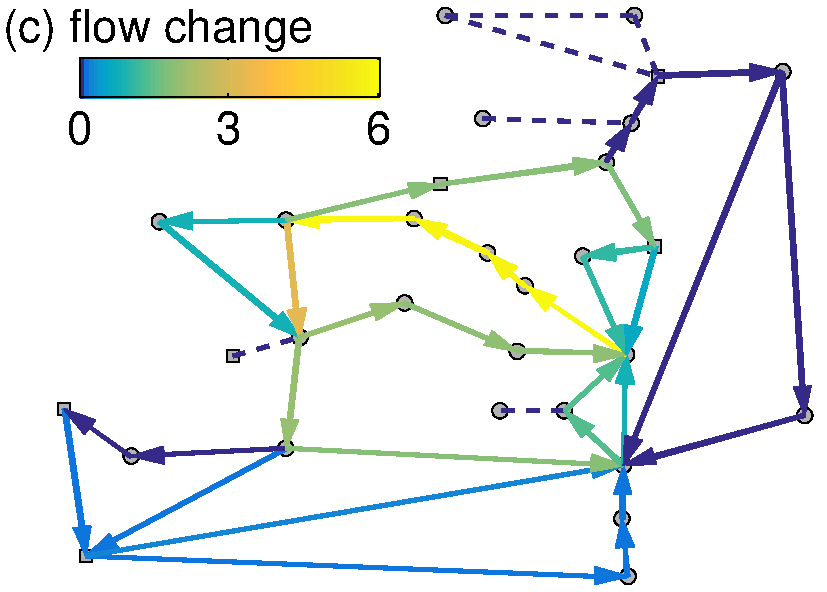
\includegraphics[width=4cm]{pics/case30c_fchange_num2.pdf} \\ [5mm]
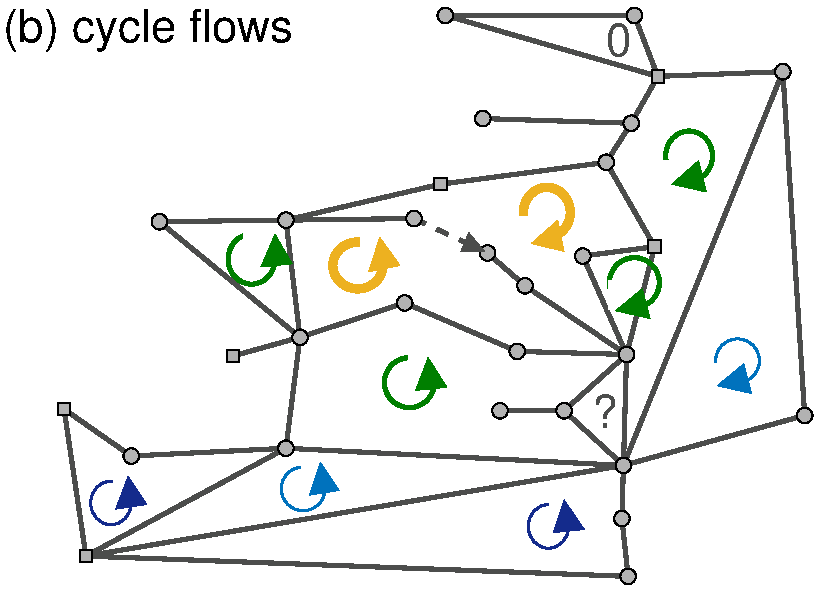
\includegraphics[width=4cm]{pics/case30c_cycles2.pdf}
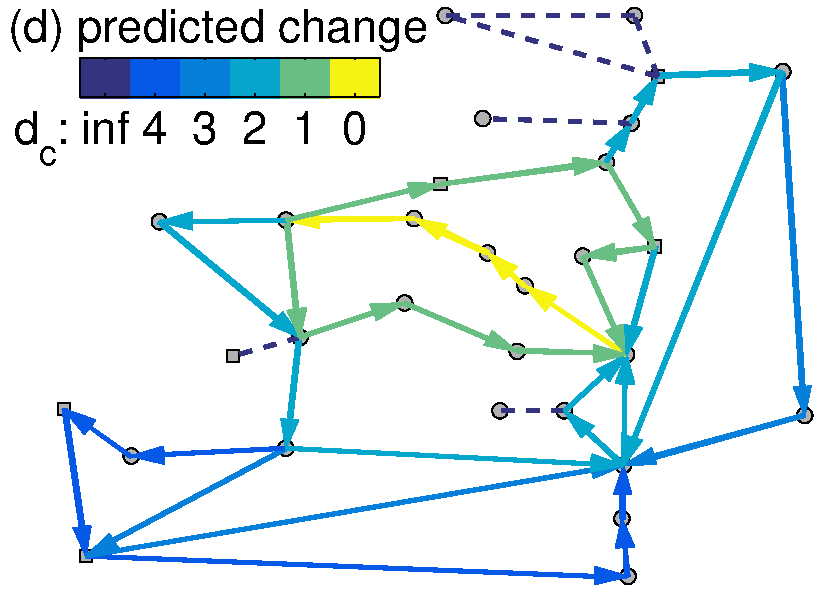
\includegraphics[width=4cm]{pics/case30c_fchange_pred2.pdf}
\caption{
\label{fig:case30}
Predicting flow changes after a transmission line failure in a model power grid.
(a) Real power flows in the initial intact network in MW.
(b) The failure of a transmission line (dashed) must be compensated by cycle flows indicated by
cyclic arrows. The thickness of the lines indicates the strength of the cycle flows. 
(c) The resulting flow changes after the failure of the marked transmission line.
(d) The direction of the flow changes are exactly predicted by algorithm \ref{thm:alg1}
for all edges and the magnitude decreases with the cycle distance $d_c$.
The power flow in (a,c) has been calculated using the standard software 
MATPOWER for the 30-bus test case \cite{MATPOWER}.
The cycle flows and the flow changes in (b,d) have been determined by algorithm 
\ref{thm:alg1}.
}
\end{figure}

\begin{figure}[tb]
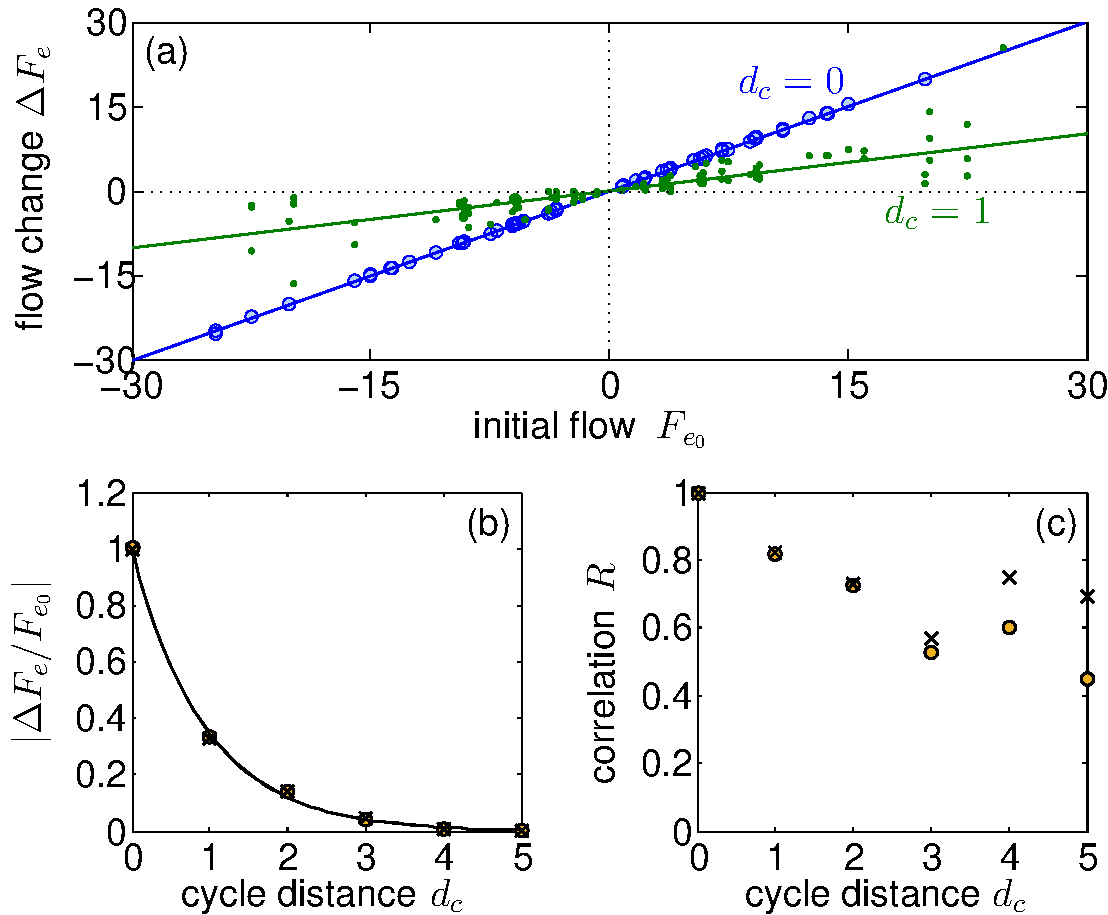
\includegraphics[width=8cm]{pics/case30d_fchange_quant2.pdf}
\caption{
\label{fig:case30q}
The reponse of a power grid to a transmission line failure increases linearly
with the flow of the failing line and decay exponentially with the cycle distance. 
(a) Flow change $\Delta F_{e}$ as a function of the initial flow of the failing
line $F_{e_0}$ for all pairs of lines $e$ and $e_1$ with cycle distance
$d_c =0$ (blue circles) and $d_c=1$ (green dots). Solid lines are linear fits.
(b) Decay of the flow change, normalized by the inital flow of the failing edge, 
with the cycle distance. Symbols are numerical values averaged over all edge
pairs with a given cycle distance $d_c$. The black line shows an exponential fit.
(c) Correlation coefficients for the linear relation in panel (a) as a function of the 
cycle distance. An almost perfect proportionality is found for $d_c=0$.
The power flow has been calculated using 
MATPOWER for the 30-bus test case \cite{MATPOWER} with the full
load flow equatiions (circles) and within the DC approximation (crosses, only
in panels b,c). Results have been collected for all pairs of failing edge $e_0$
and affected edge $e$.
}
\end{figure}

We test the algorithm for the 30 bus test grid from \cite{MATPOWER} using both the full AC load flow calculations including ohmic losses and the DC approximation. In the AC case, the voltage $U_k$ of the consumer nodes are free variables whereas the reactive power demand is fixed which yields the additional constraint \cite{Wood13} 
\be
   Q_k = \sum_{\ell=1}^{N_g+N_l} U_k U_m
            \left( G_{k m} \sin \phi_{km}-B_{k m}\cos\phi_{km} \right).   
   \label{eqn:reactivepower}
\ee  
In total, we have $2 N_g + N_l$ free variables ($N_l$ voltages and $N_g+N_l$ phase angles) to satisfy the $2 N_g + N_l$ nonlinear equations (\ref{eqn:activepower}) and (\ref{eqn:reactivepower}). Figure \ref{fig:case30} compares numerically exact values for the real power flows and the flow changes after the failure of a single transmission line with the topological predictions using algorithm \ref{thm:alg1}. The direction of the flow changes is correctly predicted for all edges. Notably, the flow changes are zero for one disconnected cycle in the north and several bridges. The strength of the flow changes depends primarily on the cycle distance to the failing edge, as shown in panels (c) and (d).

To reveal the essential factors which determine the reponse of a power grid to a local failure,
We perform a full $n-1$-simulation of the 30 bus test grid, i.e. we sample over all 
possible trigger edges and calculate the flow change for all remaining edges.
Figure \ref{fig:case30q} (a) shows that the flow change at the remaining edges depends linearly 
on the flow of the failing edge $F_{e_0}$. For a cycle distance $d_c=0$ we observe an almost
perfect proportionality while for larger distances other factors become more and more 
important. Still, we find a strong linear correlation also for larger distances, see panel (c).
The normalized flow change decays rapdily with the cycle distance as shown in panel (b). 
An exponential fit shows an excellent agreement.

In panels (b) and (c) we further compare the results of the full nonlinear load flow equation
with the lossless, linear DC approximation. Although our theory applies rigorously only to
the lossless model, we observe a very good agreement in both cases. We conclude that 
topological reponse theory yields good results also for power grids with moderate losses.

\section{Proof of proposition \ref{thm:domains}}
\label{sec:proof1}

In the following we analyze the solution of equation (\ref{eqn:cflow-lin}). W.l.o.g.  we 
assume that both the original network and the dual graph are connected. Otherwise we
can just focus on the connected component which includes the perturbed edge resp. the
perturbed cycles and exclude all disconnected parts from our analysis.

\begin{defn}
A positive domain $\DD_+$ is a connected subgraph of the dual with $f_c \ge 0$ 
for all $c \in \DD_+$ and at least one cycle with $f_c >0$. The domain $\DD_+$ is called 
isolated if $f_d \le 0$ for all cycles $d$ in the immediate neighborhood of the domain $\DD_+$. 
Analogously we use $\DD_-$ for a domain with opposite signs. 
\end{defn}

\begin{defn}
We denote by  $\mathcal{B}$ the set of edges which form the boundary of the graph, 
i.e. the set of edges which is adjacent to only one cycle in the dual graph:
\be
   \mathcal{B} = \Big\{ e \in E \Big| \sum \nolimits_{c} C_{ce} \neq 0 \Big\}.
\ee
\end{defn}

\begin{lemma}
Each isolated domain $\DD_+$ must contain a cycle $c_1$ 
with $q_{c_1} > 0$ and each isolated domain $\DD_-$ must contain a
cycle $c_2$ with $q_{c_2} < 0$.
\end{lemma}

\begin{proof}
To proof this statement assume the opposite: Let $\DD'$ be a domain with $f_c \ge 0$ 
and $\kappa q_c \le 0$ for all $c \in \DD'$ and at least one cycle with $f_c > 0$.
Using equation (\ref{eqn:cflow-lin}) we find that 
\begin{align}
    \sum_{c \in \DD'} A_{cc} f_c &= - \sum_{c \in \DD'} \sum_{d \neq c} A_{cd} f_d
           +  \sum_{c \in \DD'} \kappa q_c   \nn \\
       & =  - \sum_{c \in \DD'} \sum_{\substack{d \in \DD' \\ d \neq c}} A_{cd} f_d 
              - \sum_{c \in \DD'} \sum_{d \notin \DD'} A_{cd} f_d \nn \\
      & \qquad \qquad + \sum_{c \in \DD'} \kappa q_c .       
\end{align}
Furthermore, using the definition (\ref{eqn:def-A}) of the matrix $A$, we have
\be
    A_{cc} = - \sum_{d \neq c} A_{dc}    + \sum_{e \in \mathcal{B}} C_{ce}^2 g_e       
\ee
such that
\begin{align}
    \sum_{c \in \DD'} A_{cc} f_c 
       & =  - \sum_{c \in \DD'} \sum_{ \substack{d \in \DD' \\ d \neq c}} A_{cd} f_c 
              - \sum_{c \in \DD'} \sum_{d \notin \DD'} A_{cd} f_c \nn \\
      & \qquad \qquad + \sum_{c \in \DD'} \sum_{e \in \mathcal{B}} C_{ce}^2  \, g(F^{(0)}_e/K_e).     
\end{align}
Comparing the two expressions and using the symmetry $A_{cd} = A_{dc}$
we find that
\begin{align}
  &  - \sum_{c \in \DD'} \sum_{d \notin \DD'} A_{cd} f_d 
                + \sum_{c \in \DD'} \kappa q_c \nn \\
   & \quad =   - \sum_{c \in \DD'} \sum_{d \notin \DD'} A_{dc} f_c 
             + \sum_{c \in \DD'} \sum_{e \in \mathcal{B}} C_{ce}^2 \, g(F^{(0)}_e/K_e).
\end{align}
This leads to a contradiction as the left-hand side of the equation is smaller or 
equal to zero, while the right-hand side is larger then zero. Hence, the assumption 
must be wrong and no such domain $\DD'$ exists. 
\end{proof}

\begin{corr}
Consider the solution of equation (\ref{eqn:cflow-lin}) if exactly one edge $e_0$ is pertubed
or damaged. 

If the edge $e_0$ lies in the interior of the graph ($e_0 \notin \mathcal{B}$),
then we have $\kappa q_{c_1} > 0$ and $\kappa q_{c_2} = - \kappa q_{c_1} <0$ 
for the two cycles $c_1,c_2$ adjacent to the edge $e_0$ and $q_c = 0$ otherwise.
Then $\DD_+$ contains the cycle $c_1$ and
$\DD_-$ contains the cycle $c_2$
and no further isolated domains can exist.

If the edge $e_0$ lies on the boundary of the graph ($e_0 \in \mathcal{B}$),
then only a single cycle $c_1$ is affected with $q_{c_1} \neq 0$. Hence there is only 
one domain in the graph such that $f_c  \ge 0$ for all cycles $c$ if $q_{c_1} > 0$
and $f_c  \le 0$ for all cycles $c$ if $q_{c_1} < 0$.
\end{corr}


\section{Proof of proposition \ref{thm:decay}}
\label{sec:proof2}

As before we analyze the solution of equation (\ref{eqn:cflow-lin}) and
assume that both the original network and the dual graph are connected.
In the following we denote by $\textrm{dist}(c,c')$ the graph theoretic distance of two
vertices $c$ and $c'$ of the dual graph.

\begin{defn}
We benote by $u_d$ ($\ell_d$) the maximum (minimum) value of cycle flows  $f_c$ for all 
vertices $c$ of the dual graph with a given distance $d$ to a reference vertex $c'$:
\begin{align}
   u_d   &= \max_{c, {\rm dist}(c,c') = d}  f_c \nn \\
  \ell_d &=  \min_{c, {\rm dist}(c,c') = d}  f_c. \nn \\
\end{align}
\end{defn}

\begin{lemma}
\label{eqn:thm-monotonic}
The maximum value of the cycle flows $u_d$ decreases monotonically with the 
distance to the reference cycle $c_1$ for which $\kappa c_1 > 0$:
\begin{align}
   u_d  \le u_{d-1}, \qquad 1 \le d \le d_{\rm max}.
\end{align}
The minimum $\ell_d$ increaes monotonically with the distance to the reference 
cycle $c_2$ for which $\kappa c_2 < 0$:
\begin{align}
   \ell_d  \ge \ell_{d-1},  \qquad 1 \le d \le d_{\rm max}.
\end{align}
\end{lemma}

\begin{proof}
The proof is carried out by induction starting from $d = d_{\rm max}$. We only give
the proof for the maximum, the proof for the minimum proceeds in an analog way.

(1) Base case $d = d_{\rm max}$:
Consider the vertex $c$ of the dual for which $\textrm{dist}(c,c_1) = d_\textrm{max}$
and $f_c$ assumes its maximum $f_c = u_{d_{\rm max}}$.
Equation (\ref{eqn:cflow-lin}) yields
\begin{align}
   A_{cc}  f_c &= -  \sum \limits_{b \neq c} A_{cb} f_b  \nn \\
   &= -  \sum \limits_{\substack{b\neq c \\ \textrm{dist}(b,c_1) = d_{\rm max}}} A_{cb} f_b 
              +  \sum \limits_{\substack{b \neq c \\ \textrm{dist}(b,c_1) = d_{\rm max}-1}} A_{cb} f_b  .
              \label{eqn:proof2-f_from_ A}
\end{align}
We define the abbreviations
\begin{align}
    \mathcal{A}_d =-  \sum \limits_{b\neq c, \textrm{dist}(b,c_1) = d} A_{cb}
\end{align}
and use some important properties of the matrix $A$: 
\begin{align}
   A_{cb} & \le 0  \; \textrm{for} \, c \neq b \qquad \Rightarrow \qquad \mathcal{A}_d \ge 0 \nn \\
   A_{cc} & \ge \mathcal{A}_{d_\textrm{max}} + \mathcal{A}_{d_\textrm{max}-1}    \, .
\end{align}
We can furthermore bound the values of $f_b$ in equation (\ref{eqn:proof2-f_from_ A}) by
$u_{d_{\rm max}}$ or $u_{d_{\rm max}-1}$, resepctively, such that we obtain
\begin{align}
   u_{d_{\rm max}} = f_c  & \le 
       \frac{  \AA_{d_{\rm max}} u_{d_{\rm max}} + \AA_{d_{\rm max}-1} u_{d_{\rm max}-1} }{
                 \AA_{d_{\rm max}}  + \AA_{d_{\rm max}-1} } \nn \\
   \Rightarrow \; u_{d_{\rm max}} & \le u_{d_{\rm max}-1}, \nn \\
\end{align}

(2) Inductive step $d \rightarrow d-1$:
We consider the vertex $c$ with $\mbox{dist}(c,c_1) = d$ and $f_c = u_d$.
Staring from equation (\ref{eqn:cflow-lin}) and using the same estimations as above,
we obtain  
\begin{align}
     u_d = f_c  & = \frac{\kappa q_c - \sum_{b} A_{cb} f_b  }{A_{cc}} \nn \\
      & \le \frac{  \AA_{d-1} u_{d-1} + \AA_{d} u_{d} + \AA_{d+1} u_{d+1} }{
                 \AA_{d-1} + \AA_{d} + \AA_{d+1}} \, .\nn \\
       \label{eqn:proof2-f_from_ A2}          
\end{align}
Note that the inhomogeneity $\kappa q_c \le 0$ for all vertices except for $c = c_1$.
With the induction hypothesis $u_{d+1} \le u_d$ this yields
\begin{align}
   u_{d}   & \le \frac{  \AA_{d-1} u_{d-1} + (\AA_{d} + \AA_{d+1}) u_{d} }{
                 \AA_{d-1} + \AA_{d} + \AA_{d+1}}  \nn \\
        \Rightarrow u_d & \le u_{d-1}.
\end{align}
which completes the proof.    
\end{proof}

\begin{lemma}
The maximum (minimum) value of the cycle flows $u_d$ decreases (increases) \emph{strictly} 
monotonically with the distance to the reference cycle $c_1$ ($c_2$)
\begin{align}
   u_d  &< u_{d-1},  \nn \\
   \ell_d  &> \ell_{d-1},  \qquad 1 \le d \le d_{\rm max}.
\end{align}
if (1) all cycles $c$ at maximum distance from $c_1$ lie at the boundary of the dual graph,
\begin{align}
  & \forall c \; {\rm with} \, {\rm dist}(c,c_1) = d_{\rm max}: \\
  & \qquad  \exists \,  {\rm edge} \, e \; {\rm with} \; e \in \mathcal{B} \; {\rm and} \;
     C_{ce} \neq 0. 
\end{align}
or (2) all extrema $u_d$ and $\ell_d$ are unique.  
\end{lemma}

\begin{proof}
We show that in both cases we can replace $\ge$ by $>$ in the base case and thus also
in the inductive step in the proof of lemma \ref{eqn:thm-monotonic}.
If condition (1) is satisfied we have 
\be
     A_{cc}  > \mathcal{A}_{d_\textrm{max}} + \mathcal{A}_{d_\textrm{max}-1}  
\ee
due to boundary terms.
If condition (1) is not satisfied but 
condition (2) is, then the sum in equation \ref{eqn:proof2-f_from_ A} includes at least two terms.
One of the values of $f_b$ in the sum must be strictly smaller than the maximum value
$u_d$ or $u_{d-1}$, respectively, as we assumed that these maxima are unique. We thus
can replace the $\ge$ by $<$ in the estimations.


\end{proof}


\section{Decay in regular lattices}
\label{sec:proof-regular}
\begin{figure}
    \begin{center}
        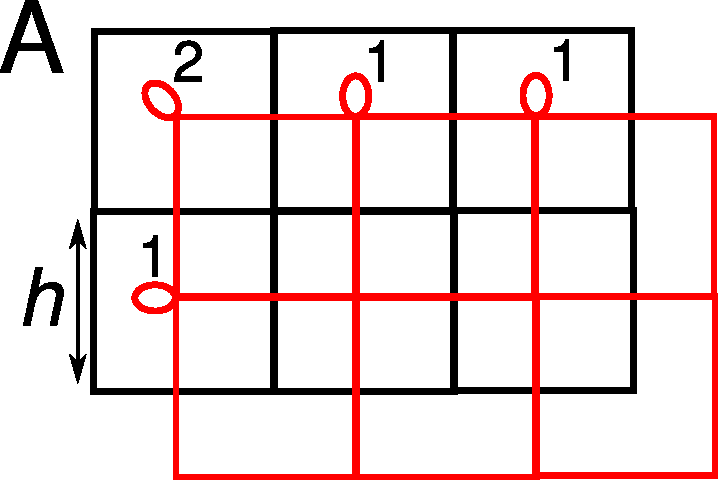
\includegraphics[width=0.2\textwidth]{pics/DualLattice.pdf} \quad
        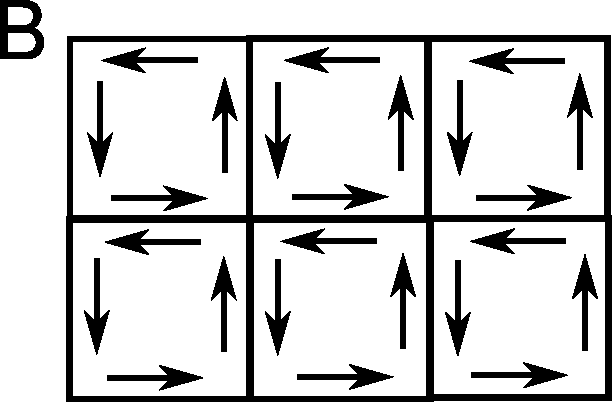
\includegraphics[width=0.2\textwidth]{pics/OrientedCycles.pdf}
    \end{center}
    \caption{A. A square lattice (black) together with its cycle-dual
    (red).
    The cycle dual is also a square lattice, but because the boundary
    edges are only adjacent to one cycle, it contains self-loops
    at its boundary nodes. The weight of a self loop is the sum
    of all boundary edge weights which are part of the boundary cycle.
    In the limit $h\rightarrow 0$, the self-loops enforce Dirichlet
    boundary conditions on the cycle density, $\phi|_{\partial A} = 0$.
    B. Consistently oriented cycles in a square lattice.
    \label{fig:cycles-lattice}}
\end{figure}
In this appendix we derive the continuum model directly from the discrete
network model in the uniform case. Consider a network with
cycle edge adjacency matrix $C_{ce}$. Then we are interested in a
continuous version of equation (\ref{eqn:cflow-lin}).
On a square lattice the application of $A_{cd}$ to a vector in the 
bulk can be written, going to the continuous limit (see Fig. \ref{fig:cycles-lattice}),
\begin{align}
    (A\phi)(x) &= \frac{\phi(x,y)}{K(x + h/2,y)} 
    +\frac{\phi(x,y)}{K(x - h/2,y)} \\
    &\quad+ \frac{\phi(x,y)}{K(x,y+h/2)}
    + \frac{\phi(x,y)}{K(x,y-h/2)} \\
    &\quad -\frac{\phi(x+h,y)}{K(x+h/2,y)}
    -\frac{\phi(x-h,y)}{K(x-h/2,y)} \\
    &\quad-\frac{\phi(x,y+h)}{K(x,y+h/2)}
    -\frac{\phi(x,y-h)}{K(x,y-h/2)} \\
    &= h^2 \nabla \cdot \left(\frac{1}{K} \nabla \phi\right) + O(h^3).
\end{align}
Here, $h$ is the lattice spacing.
The right hand side works similarly, noting that only two cycles
contribute, with opposite signs. Let us assume that $e_0$ is
parallel to the $y$ axis. Then the RHS is
\begin{align}
    &- v_y(x+h/2,y) \frac{\kappa}{K(x+h/2,y)(K(x+h/2,y)-\kappa)} \\
    &\quad \times \delta^{(2)}(x+h/2,y)
    \\
    &\quad+ v_y(x-h/2,y) \frac{\kappa}{K(x-h/2,y)(K(x-h/2,y)-\kappa)} \\
    &\quad\times \delta^{(2)}(x-h/2,y)
    \\
    &= h \frac{\partial}{\partial x} \left(v_y
    \frac{\kappa}{K(K-\kappa)}\delta^{(2)}(x,y)\right) + O(h^3).
\end{align}
This is a dipole source field with dipole moment parallel to the 
$x$ axis. It is easy to see the generalization to arbitrary dipole
moments. Thus, the full continuous equations governing the behaviour
of the cycle density in the bulk are
\begin{align}
 \nabla \cdot \left(\frac{1}{K} \nabla \phi\right) =
 -\vec p \cdot \nabla \delta^{(2)}(\vec x-\vec a),
 \label{eqn:dipole}
\end{align}
for a perturbation at $\vec a$. The dipole vector $\vec p$ is
orthogonal in direction to flow at the site of perturbation and
proportional in magnitude.
More perturbations can be handled
by linear combination. Note that we have subsumed
the factors of $h$ into the derivative by a change of variables
$\vec x \rightarrow h \vec x$.

At the boundary, a similar relation as in the bulk holds, supplying us
with boundary conditions.
Because boundary cycles
possess three neighboring cycles four edges in total, some
terms are left over;
\begin{align}
    (A\phi)(x) &= \frac{\phi(x,y)}{K(x + h/2,y)} 
    +\frac{\phi(x,y)}{K(x - h/2,y)} \\
    &\quad + \frac{\phi(x,y)}{K(x,y+h/2)}
    + \frac{\phi(x,y)}{K(x,y-h/2)} \\
    &\quad -\frac{\phi(x+h,y)}{K(x+h/2,y)}
    -\frac{\phi(x-h,y)}{K(x-h/2,y)} \\
    &\quad -\frac{\phi(x,y-h)}{K(x,y-h/2)} \\
    &= \frac{\phi(x,y)}{K(x,y)} + O(h).
\end{align}
Thus, we find that Dirichlet boundary conditions must hold in the absence
of boundary perturbations:
$\phi|_{\partial A} = 0$.

Finally, we need a law telling us how to calculate a flow vector
from the cycle density. To this end, consider 
Figure \ref{fig:cycles-lattice} B. In order to obtain the $y$ component
of a flow vector, we need to add up the contributions of two cycle
flows neighboring in the $x$ direction, and vice versa. Thus,
the flow vector becomes
\begin{align}
    \vec v(\vec x) &= \begin{pmatrix}
        \phi(x,y+h/2) - \phi(x, y-h/2) \\
        \phi(x-h/2,y) - \phi(x+h/2,y)
    \end{pmatrix} \\
    &= \begin{pmatrix}
        0 & 1 \\
        -1 & 0
    \end{pmatrix} \nabla \phi + O(h),
\end{align}
where we again rescaled $\vec x\rightarrow h \vec x$.

In the case of uniform conductivity density $K(\vec x) \equiv K$,
equation (\ref{eqn:dipole}) becomes a regular Poisson equation
in two dimensions with dipole source density. The solutions
to this equation are well known from the theory of electrostatics, 
on an infinite domain taking the form
\begin{align}
    \phi(\vec x) &= \frac{\vec p \cdot \vec x}{\vec x^2} \\
    \vec v(\vec x) &= \begin{pmatrix} 0 & 1 \\ -1 & 0 \end{pmatrix}
        \left( \frac{\vec p}{\vec x^2} - 2 \vec x \frac{\vec p \cdot
             \vec x}{\vec x^4} \right)
\end{align}
for a perturbation at $\vec a = 0$.
Indeed, the cycle density decays as $\phi(r) \sim r^{-1}$ and 
the flow due to the perturbation as $\vec v(r) \sim r^{-2}$.






\section{Relationship between cycle flow and resistance distance}
\label{sec:resdist}

For linear flows, as discussed in \ref{sec:linflow-planar}, the equation \eqref{eqn:cflow-lin} 
governing cycle flows 
\begin{align}
   \label{eq:lapl-lin}
   A f_c &= \kappa q_d
\end{align}
is exact and equation \eqref{eqn:def-A} for the matrix $A$ simplifies to
\begin{align}
   A_{d,c} &= \sum_{e=1}^L C_{d,e} C_{c,e} \\
           &=
	     \begin{cases}
	     \text{No. of edges shared by faces c and d} & \text{if } c\neq d\\
	     \text{No. of edges in face c} & \text{if } c=d.
	     \end{cases}
    \nonumber	     
\end{align}
Then the matrix $A$ can be seen as a part of the Laplacian of the dual Graph 
of $G$, the original network.  
Let $L$ be a full Laplacian of the dual graph $D(G)$, whose $1$st row 
corresponds to the \emph{unbounded face} of $G$.  Then $A$ can 
be simply obtained by deleting the first row and first column of $L$.  
\begin{align*}
L&=
\left(
\begin{array}{c|ccc}
L_{11} & L_{12} & L_{13} & \cdots \\
\hline
L_{21} &&&\\
L_{31} && A &\\
L_{41} &&&         
\end{array}
\right)
\end{align*}

\dirk{XXX @ Debsankha: Please add a reference for the definition of the Laplacian of a
dual graph. And cite Newmann, networks for Laplacians in general. XXX} \cite{Newm10}

Now, equation \eqref{eq:lapl-lin} is equivalent to the the auxiliary equation
\begin{align}
\label{eq:aux-lin}
L f' &= \kappa q_d'\\
f'[1]&= 0
\end{align}
where $q_d'=0\otimes q_d$.  This equation can be formally solved as 
\begin{align}
  \label{eq:sol-lg}
   f'&=\kappa L^+ q_d',
\end{align}
Where $L^+$ is the Moore-Penrose pseudoinverse of $L$. 
Now, the Moore-Penrose pseudoinverse is closely related to the resistance distance,
which provides a metric on graphs \cite{Klei93}. In particular, the elements of 
$L^+$ are given by
\begin{align*}
   L^+_{ij}&=-\frac{R_{ij}}{2}+\frac{1}{2|V|} \left( R_i^{\rm tot}+R_j^{\rm tot} \right)
\end{align*}
where $R_{ij}$ is the resistance distance between the faces $i$ and $j$ and 
$R_i^{\rm tot}$ is \dirk{XXX @ Debsankha: what? XXX}
Pluggingt these realtions into equation \eqref{eq:sol-lg}, we obtain
\begin{align*}
   f_c &= \kappa \left(R_{c,c_0}-R_{c,c_1}\right) + \text{ const}
\end{align*}

% --- Literatur -------------------------------------------------------------------

\bibliography{cycle}
\bibliographystyle{apsrev}




\end{document}




